\documentclass{book}

\usepackage[activeacute, spanish]{babel}
\spanishdecimal{.} % usar puntos en vez de comas en modo matematico
\usepackage[utf8]{inputenc}

\usepackage[sc]{mathpazo} % Usar fuente Palatino
\usepackage[T1]{fontenc} % Usar codigicacion 8-bit
\linespread{1.05} % Espacio de linea - Palatino necesita mas espacio entre lineas
\usepackage{microtype} % Ajustar ligeramente el espaciado de letra
                       % para la estética

\usepackage{makeidx}
\usepackage[hidelinks]{hyperref} % hidelinks elimina el recuadro en los enlaces
\usepackage{graphicx} % Requerido para insertar imagenes
\usepackage{eso-pic}     %permite poner una imagen de fondo
\newcommand\imgFondo{%
   \put(0,0){%
     \parbox[b][\paperheight]{\paperwidth}{%
       \vfill
       \centering
       \includegraphics{img/f.png}%
       \vfill
}}}
\usepackage{float}
\usepackage[left=2cm,top=2cm,right=2cm,bottom=2cm]{geometry} % Margenes

% ------------------------- ini-meta.tex -------------------------
\usepackage{hyperref} %requerido para \hypersetup
\hypersetup{
  pdftitle={Tareas matematica aplicada 3, FIUSAC},
  pdfauthor={Wilson S. Tubin},
  pdfsubject={WeGT},
  pdfcreator={https://wilsoneliseo.wordpress.com/},
  pdfproducer={https://wilsoneliseo.wordpress.com/},
  pdfkeywords={WeGT}
}
% ------------------------- fin-meta.tex -------------------------
\author{Wilson S. Tubín \\ wilsoneliseogt@gmail.com}
\title{Ejercicios, métodos numéricos. \\FIUSAC}
\date{}


\begin{document}
\AddToShipoutPictureBG{\imgFondo}
\maketitle

Los ejercicios fueron tomados de libro titulado <<Análisis Numérico>> 
novena edicion de Richard L. Burden y J. Douglas Faires.


\chapter{Biseccion \\ 
{\normalsize Ejercicios de Seccion 2.1, Pág. 54 }
}
\section{ejercicio 2}
\par Sea $
f\left(x\right):=3\,\left(x+1\right)\,\left(x-\frac{1}{2}\right)\,\left(x-1\right)
$. Use el método de bisección para encontrar $p_3$ en los siguientes
intervalos.
\begin{itemize}
\item[a)] $[-2, 1.5]$
\item[b)] $[-1.25, 2.5]$
\end{itemize}

\subsection{inciso a)}
\begin{verbatim}
  $ biseccion(-2,1.5,5,3);
\end{verbatim}

\[
  \pmatrix{N&a&b&p&\mathrm{f}\left(a\right)&\mathrm{f}\left(b\right)&\mathrm{f}\left(p\right)&\mathrm{f}\left(a\right)
    * \mathrm{f}\left(p\right)&\mathrm{error}\cr
    1&-2&1.5&-0.25&-22.5&3.75&2.109375&-47.4609375&1.75\cr
    2&-2&-0.25&-1.125&-22.5&2.109375&-1.2949219&29.1357428&0.875\cr
    3&-1.125&-0.25&-0.6875&-1.2949219&2.109375&1.8786621&-2.4327207&0.4375\cr
  }
\]

\subsection{inciso b)}
\begin{verbatim}
  biseccion(-1.25,2.5,5,3);
\end{verbatim}

\[
  \pmatrix{N&a&b&p&\mathrm{f}\left(a\right)&\mathrm{f}\left(b\right)&\mathrm{f}\left(p\right)&\mathrm{f}\left(a\right)
    * \mathrm{f}\left(p\right)&\mathrm{error}\cr
    1&-1.25&2.5&0.625&-2.953125&31.5&-0.2285156&0.6748351&1.875\cr
    2&0.625&2.5&1.5625&-0.2285156&31.5&4.5944824&-1.0499109&0.9375\cr
    3&0.625&1.5625&1.09375&-0.2285156&4.5944824&0.3496399&-0.0798982&0.46875\cr
  }
\]

\section{ejercicio 3}
\par Use el método de biseccion para encontrar la solución de $
f\left(x\right):=x^3-7\,x^2+14\,x-6$ con una toleracia de $10^{-2}$

\subsection{inciso b)}
En el intervalo $[1,3.2]$

\begin{verbatim}
  f(x):=x^3-7*x^2+14*x-6;
  biseccion(1,3.2,2,20);
\end{verbatim}

$$
\pmatrix{N&a&b&p&f\left(a\right)&f\left(b\right)&f\left(p\right)&f
 \left(a\right)\,f\left(p\right)&{\it error}\cr 1&1&3.2&2.1&2&-0.112&
 1.791&3.582&1.1\cr 2&2.1&3.2&2.65&1.791&-0.112&0.552&0.989&0.55\cr 3
 &2.65&3.2&2.925&0.552&-0.112&0.0858&0.0474&0.275\cr 4&2.925&3.2&
 3.0625&0.0858&-0.112&-0.0544&-0.00467&0.137\cr 5&2.925&3.0625&2.9938
 &0.0858&-0.0544&0.00633&5.4311 \times 10^{-4}&0.0687\cr 6&2.9938&
 3.0625&3.0281&0.00633&-0.0544&-0.0265&-1.6782 \times 10^{-4}&0.0344
 \cr 7&2.9938&3.0281&3.0109&0.00633&-0.0265&-0.0107&-
 6.76889 \times 10^{-5}&0.0172\cr 8&2.9938&3.0109&3.0023&0.00633&-
 0.0107&-0.00233&-1.47614 \times 10^{-5}&0.00859\cr }
$$

\section{ejercicio 5}
\par Use el metodo de biseccion para encontrar la solución, de los
siguientes, con una tolerancia de $10^{-5}$

\subsection{inciso a)}
La funcion $f(x):=x-2^{-x}$ en el intervalo $[0,1]$

\begin{verbatim}
  f(x):=x-2^(-x);
  biseccion(0, 1, 5, 20);
\end{verbatim}

{\scriptsize
$$\pmatrix{N&a&b&p&f\left(a\right)&f\left(b\right)&f\left(p\right)&f
 \left(a\right)\,f\left(p\right)&{\it error}\cr 1&0&1&0.5&-1&0.5&-
 0.207107&0.207107&0.5\cr 2&0.5&1&0.75&-0.207107&0.5&0.155396&-
 0.0321837&0.25\cr 3&0.5&0.75&0.625&-0.207107&0.155396&-0.0234198&
 0.00485039&0.125\cr 4&0.625&0.75&0.6875&-0.0234198&0.155396&
 0.0665711&-0.00155908&0.0625\cr 5&0.625&0.6875&0.65625&-0.0234198&
 0.0665711&0.0217245&-5.08783454 \times 10^{-4}&0.03125\cr 6&0.625&
 0.65625&0.640625&-0.0234198&0.0217245&-8.10008039 \times 10^{-4}&
 1.89702079 \times 10^{-5}&0.015625\cr 7&0.640625&0.65625&0.648438&-
 8.10008039 \times 10^{-4}&0.0217245&0.0104666&-
 8.47803889 \times 10^{-6}&0.0078125\cr 8&0.640625&0.648438&0.644531&
 -8.10008039 \times 10^{-4}&0.0104666&0.00483065&-
 3.9128623 \times 10^{-6}&0.00390625\cr 9&0.640625&0.644531&0.642578&
 -8.10008039 \times 10^{-4}&0.00483065&0.00201091&-
 1.62885012 \times 10^{-6}&0.00195313\cr 10&0.640625&0.642578&
 0.641602&-8.10008039 \times 10^{-4}&0.00201091&
 6.00595889 \times 10^{-4}&-4.86487499 \times 10^{-7}&
 9.765625 \times 10^{-4}\cr 11&0.640625&0.641602&0.641113&-
 8.10008039 \times 10^{-4}&6.00595889 \times 10^{-4}&-
 1.0466935 \times 10^{-4}&8.47830146 \times 10^{-8}&
 4.8828125 \times 10^{-4}\cr 12&0.641113&0.641602&0.641357&-
 1.0466935 \times 10^{-4}&6.00595889 \times 10^{-4}&
 2.4797245 \times 10^{-4}&-2.5955115 \times 10^{-8}&
 2.44140625 \times 10^{-4}\cr 13&0.641113&0.641357&0.641235&-
 1.0466935 \times 10^{-4}&2.4797245 \times 10^{-4}&
 7.16538452 \times 10^{-5}&-7.49996137 \times 10^{-9}&
 1.22070313 \times 10^{-4}\cr 14&0.641113&0.641235&0.641174&-
 1.0466935 \times 10^{-4}&7.16538452 \times 10^{-5}&-
 1.65071784 \times 10^{-5}&1.72779562 \times 10^{-9}&
 6.10351563 \times 10^{-5}\cr 15&0.641174&0.641235&0.641205&-
 1.65071784 \times 10^{-5}&7.16538452 \times 10^{-5}&
 2.75734769 \times 10^{-5}&-4.55160301 \times 10^{-10}&
 3.05175781 \times 10^{-5}\cr 16&0.641174&0.641205&0.64119&-
 1.65071784 \times 10^{-5}&2.75734769 \times 10^{-5}&
 5.5331851 \times 10^{-6}&-9.13372735 \times 10^{-11}&
 1.52587891 \times 10^{-5}\cr 17&0.641174&0.64119&0.641182&-
 1.65071784 \times 10^{-5}&5.5331851 \times 10^{-6}&-
 5.48698768 \times 10^{-6}&9.05746843 \times 10^{-11}&
 7.62939453 \times 10^{-6}\cr }$$
}

\subsection{inciso c)}
\par En el intervalo $[-3, -2]$ y $[-1, 0]$ con la funcion $
f\left(x\right):=2\,x\,\cos
\left(2\,x\right)-\left(x+1\right)^2$

\subsubsection{intervalo [-3, -2]}

\begin{verbatim}
  f(x):=2*x*cos(2*x)-(x+1)^2;
  biseccion(-3, -2, 5, 20);
\end{verbatim}


{\tiny
$$\pmatrix{N&a&b&p&f\left(a\right)&f\left(b\right)&f\left(p\right)&f
 \left(a\right)\,f\left(p\right)&{\it error}\cr 1&-3&-2&-2.5&-
 9.7610217&1.6145745&-3.6683109&35.806463&0.5\cr 2&-2.5&-2&-2.25&-
 3.6683109&1.6145745&-0.613919&2.2520454&0.25\cr 3&-2.25&-2&-2.125&-
 0.613919&1.6145745&0.630247&-0.38692&0.125\cr 4&-2.25&-2.125&-2.1875
 &-0.613919&0.630247&0.0380755&-0.0233753&0.0625\cr 5&-2.25&-2.1875&-
 2.21875&-0.613919&0.0380755&-0.280836&0.172411&0.03125\cr 6&-2.21875
 &-2.1875&-2.203125&-0.280836&0.0380755&-0.119557&0.0335759&0.015625
 \cr 7&-2.203125&-2.1875&-2.1953125&-0.119557&0.0380755&-0.0402785&
 0.00481557&0.0078125\cr 8&-2.1953125&-2.1875&-2.1914063&-0.0402785&
 0.0380755&-9.85194952 \times 10^{-4}&3.96821888 \times 10^{-5}&
 0.00390625\cr 9&-2.1914063&-2.1875&-2.1894531&-
 9.85194952 \times 10^{-4}&0.0380755&0.0185743&-
 1.8299343 \times 10^{-5}&0.00195313\cr 10&-2.1914063&-2.1894531&-
 2.1904297&-9.85194952 \times 10^{-4}&0.0185743&0.00880185&-
 8.67153955 \times 10^{-6}&9.765625 \times 10^{-4}\cr 11&-2.1914063&-
 2.1904297&-2.190918&-9.85194952 \times 10^{-4}&0.00880185&0.00391015
 &-3.85225692 \times 10^{-6}&4.8828125 \times 10^{-4}\cr 12&-
 2.1914063&-2.190918&-2.1911621&-9.85194952 \times 10^{-4}&0.00391015
 &0.00146293&-1.44127166 \times 10^{-6}&2.44140625 \times 10^{-4}\cr 
 13&-2.1914063&-2.1911621&-2.1912842&-9.85194952 \times 10^{-4}&
 0.00146293&2.38981324 \times 10^{-4}&-2.35443194 \times 10^{-7}&
 1.22070313 \times 10^{-4}\cr 14&-2.1914063&-2.1912842&-2.1913452&-
 9.85194952 \times 10^{-4}&2.38981324 \times 10^{-4}&-
 3.73078418 \times 10^{-4}&3.67554975 \times 10^{-7}&
 6.10351563 \times 10^{-5}\cr 15&-2.1913452&-2.1912842&-2.1913147&-
 3.73078418 \times 10^{-4}&2.38981324 \times 10^{-4}&-
 6.70414481 \times 10^{-5}&2.50117174 \times 10^{-8}&
 3.05175781 \times 10^{-5}\cr 16&-2.1913147&-2.1912842&-2.1912994&-
 6.70414481 \times 10^{-5}&2.38981324 \times 10^{-4}&
 8.59717127 \times 10^{-5}&-5.76366811 \times 10^{-9}&
 1.52587891 \times 10^{-5}\cr 17&-2.1913147&-2.1912994&-2.1913071&-
 6.70414481 \times 10^{-5}&8.59717127 \times 10^{-5}&
 9.46557602 \times 10^{-6}&-6.34585923 \times 10^{-10}&
 7.62939453 \times 10^{-6}\cr }$$
}

\subsubsection{intervalo [-1, 0]}

\begin{verbatim}
  f(x):=2*x*cos(2*x)-(x+1)^2;
  biseccion(-1, 0, 5, 20);
\end{verbatim}


{\tiny
$$\pmatrix{N&a&b&p&f\left(a\right)&f\left(b\right)&f\left(p\right)&f
 \left(a\right)\,f\left(p\right)&{\it error}\cr 1&-1&0&-0.5&0.832294&
 -1&-0.790302&-0.657764&0.5\cr 2&-1&-0.5&-0.75&0.832294&-0.790302&-
 0.168606&-0.14033&0.25\cr 3&-1&-0.75&-0.875&0.832294&-0.168606&
 0.296306&0.246613&0.125\cr 4&-0.875&-0.75&-0.8125&0.296306&-0.168606
 &0.0528816&0.0156691&0.0625\cr 5&-0.8125&-0.75&-0.78125&0.0528816&-
 0.168606&-0.0608144&-0.00321596&0.03125\cr 6&-0.8125&-0.78125&-
 0.796875&0.0528816&-0.0608144&-0.00468056&-2.47515541 \times 10^{-4}
 &0.015625\cr 7&-0.8125&-0.796875&-0.804688&0.0528816&-0.00468056&
 0.0239252&0.0012652&0.0078125\cr 8&-0.804688&-0.796875&-0.800781&
 0.0239252&-0.00468056&0.00957807&2.29156947 \times 10^{-4}&
 0.00390625\cr 9&-0.800781&-0.796875&-0.798828&0.00957807&-0.00468056
 &0.00243764&2.33478872 \times 10^{-5}&0.00195313\cr 10&-0.798828&-
 0.796875&-0.797852&0.00243764&-0.00468056&-0.00112424&-
 2.74050365 \times 10^{-6}&9.765625 \times 10^{-4}\cr 11&-0.798828&-
 0.797852&-0.79834&0.00243764&-0.00112424&6.56003277 \times 10^{-4}&
 1.59910056 \times 10^{-6}&4.8828125 \times 10^{-4}\cr 12&-0.79834&-
 0.797852&-0.798096&6.56003277 \times 10^{-4}&-0.00112424&-
 2.34294318 \times 10^{-4}&-1.5369784 \times 10^{-7}&
 2.44140625 \times 10^{-4}\cr 13&-0.79834&-0.798096&-0.798218&
 6.56003277 \times 10^{-4}&-2.34294318 \times 10^{-4}&
 2.10811015 \times 10^{-4}&1.38292717 \times 10^{-7}&
 1.22070313 \times 10^{-4}\cr 14&-0.798218&-0.798096&-0.798157&
 2.10811015 \times 10^{-4}&-2.34294318 \times 10^{-4}&-
 1.17525187 \times 10^{-5}&-2.47756039 \times 10^{-9}&
 6.10351563 \times 10^{-5}\cr 15&-0.798218&-0.798157&-0.798187&
 2.10811015 \times 10^{-4}&-1.17525187 \times 10^{-5}&
 9.95265316 \times 10^{-5}&2.09812892 \times 10^{-8}&
 3.05175781 \times 10^{-5}\cr 16&-0.798187&-0.798157&-0.798172&
 9.95265316 \times 10^{-5}&-1.17525187 \times 10^{-5}&
 4.38863273 \times 10^{-5}&4.36785394 \times 10^{-9}&
 1.52587891 \times 10^{-5}\cr 17&-0.798172&-0.798157&-0.798164&
 4.38863273 \times 10^{-5}&-1.17525187 \times 10^{-5}&
 1.60667345 \times 10^{-5}&7.05109969 \times 10^{-10}&
 7.62939453 \times 10^{-6}\cr }$$
}

\section{ejercicio 7}

\subsection{inciso a)}
Grafique $y=x$ y $y=2*sin(x)$ en un mismo cuadro.

\begin{verbatim}
  wxplot2d([x,2*sin(x)],[x,-5,5]);
\end{verbatim}

\begin{figure}[H]
  \centering
  \includegraphics[scale=0.45]{img/maxout_1.eps}
\end{figure}

\subsection{inciso b)}
\begin{verbatim}
  f(x):=2*sin(x);
  biseccion(3.05, 3.2, 5, 20);
\end{verbatim}

{\scriptsize
$$\pmatrix{N&a&b&p&f\left(a\right)&f\left(b\right)&f\left(p\right)&f
 \left(a\right)\,f\left(p\right)&{\it error}\cr 1&3.05&3.2&3.125&
 0.182929&-0.116748&0.0331838&0.00607029&0.075\cr 2&3.125&3.2&3.1625&
 0.0331838&-0.116748&-0.0418116&-0.00138747&0.0375\cr 3&3.125&3.1625&
 3.14375&0.0331838&-0.0418116&-0.00431469&-1.43177725 \times 10^{-4}&
 0.01875\cr 4&3.125&3.14375&3.134375&0.0331838&-0.00431469&0.0144352&
 4.79013963 \times 10^{-4}&0.009375\cr 5&3.134375&3.14375&3.1390625&
 0.0144352&-0.00431469&0.0050603&7.30463764 \times 10^{-5}&0.0046875
 \cr 6&3.1390625&3.14375&3.1414062&0.0050603&-0.00431469&
 3.72807177 \times 10^{-4}&1.88651682 \times 10^{-6}&0.00234375\cr 7&
 3.1414062&3.14375&3.1425781&3.72807177 \times 10^{-4}&-0.00431469&-
 0.00197094&-7.34781511 \times 10^{-7}&0.00117188\cr 8&3.1414062&
 3.1425781&3.1419922&3.72807177 \times 10^{-4}&-0.00197094&-
 7.99067799 \times 10^{-4}&-2.97898211 \times 10^{-7}&
 5.859375 \times 10^{-4}\cr 9&3.1414062&3.1419922&3.1416992&
 3.72807177 \times 10^{-4}&-7.99067799 \times 10^{-4}&-
 2.1313032 \times 10^{-4}&-7.9456513 \times 10^{-8}&
 2.9296875 \times 10^{-4}\cr 10&3.1414062&3.1416992&3.1415527&
 3.72807177 \times 10^{-4}&-2.1313032 \times 10^{-4}&
 7.98384296 \times 10^{-5}&2.97643396 \times 10^{-8}&
 1.46484375 \times 10^{-4}\cr 11&3.1415527&3.1416992&3.141626&
 7.98384296 \times 10^{-5}&-2.1313032 \times 10^{-4}&-
 6.66459454 \times 10^{-5}&-5.32090762 \times 10^{-9}&
 7.32421875 \times 10^{-5}\cr 12&3.1415527&3.141626&3.1415894&
 7.98384296 \times 10^{-5}&-6.66459454 \times 10^{-5}&
 6.59624209 \times 10^{-6}&5.26633609 \times 10^{-10}&
 3.66210937 \times 10^{-5}\cr 13&3.1415894&3.141626&3.1416077&
 6.59624209 \times 10^{-6}&-6.66459454 \times 10^{-5}&-
 3.00248517 \times 10^{-5}&-1.9805119 \times 10^{-10}&
 1.83105469 \times 10^{-5}\cr 14&3.1415894&3.1416077&3.1415985&
 6.59624209 \times 10^{-6}&-3.00248517 \times 10^{-5}&-
 1.17143048 \times 10^{-5}&-7.72703903 \times 10^{-11}&
 9.15527344 \times 10^{-6}\cr }$$
}

\section{ejercicio 9}

\subsection{inciso a)}
Grafique $y=e^x-2$ y $y=cos(e-2)$ en un mismo cuadro

\begin{verbatim}
  wxplot2d([%e^x-2,cos(%e^x-2)],[x,0,3]);
\end{verbatim}

\begin{figure}[H]
  \centering
  \includegraphics[scale=0.45]{img/maxout_3.eps}
\end{figure}


\subsection{inciso b)}
Use el método de biseccion para aproximar la intersección
$e^x-2=\cos\left(e-2\right)$ en el intervalo $[0.5, 1.5]$ con una
tolerancia $10^{-5}$

\begin{verbatim}
  f(x):=cos(%e-2)-%e^x+2;
  biseccion(0.5, 1.5, 5, 20);
\end{verbatim}


{\tiny
$$\pmatrix{N&a&b&p&f\left(a\right)&f\left(b\right)&f\left(p\right)&f
 \left(a\right)\,f\left(p\right)&{\it error}\cr 1&0.5&1.5&1.0&
 1.1042163&-1.7287515&0.0346557&0.0382674&0.5\cr 2&1.0&1.5&1.25&
 0.0346557&-1.7287515&-0.737405&-0.0255553&0.25\cr 3&1.0&1.25&1.125&
 0.0346557&-0.737405&-0.327279&-0.0113421&0.125\cr 4&1.0&1.125&1.0625
 &0.0346557&-0.327279&-0.140658&-0.00487462&0.0625\cr 5&1.0&1.0625&
 1.03125&0.0346557&-0.140658&-0.0516318&-0.00178934&0.03125\cr 6&1.0&
 1.03125&1.015625&0.0346557&-0.0516318&-0.00815098&-
 2.82478261 \times 10^{-4}&0.015625\cr 7&1.0&1.015625&1.0078125&
 0.0346557&-0.00815098&0.013336&4.62167997 \times 10^{-4}&0.0078125
 \cr 8&1.0078125&1.015625&1.0117188&0.013336&-0.00815098&0.00261348&
 3.48533162 \times 10^{-5}&0.00390625\cr 9&1.0117188&1.015625&
 1.0136719&0.00261348&-0.00815098&-0.0027635&-
 7.22234146 \times 10^{-6}&0.00195313\cr 10&1.0117188&1.0136719&
 1.0126953&0.00261348&-0.0027635&-7.36948619 \times 10^{-5}&-
 1.92600075 \times 10^{-7}&9.765625 \times 10^{-4}\cr 11&1.0117188&
 1.0126953&1.012207&0.00261348&-7.36948619 \times 10^{-5}&0.00127022&
 3.31969708 \times 10^{-6}&4.8828125 \times 10^{-4}\cr 12&1.012207&
 1.0126953&1.0124512&0.00127022&-7.36948619 \times 10^{-5}&
 5.98344986 \times 10^{-4}&7.60030235 \times 10^{-7}&
 2.44140625 \times 10^{-4}\cr 13&1.0124512&1.0126953&1.0125732&
 5.98344986 \times 10^{-4}&-7.36948619 \times 10^{-5}&
 2.62345571 \times 10^{-4}&1.56973157 \times 10^{-7}&
 1.22070313 \times 10^{-4}\cr 14&1.0125732&1.0126953&1.0126343&
 2.62345571 \times 10^{-4}&-7.36948619 \times 10^{-5}&
 9.43304821 \times 10^{-5}&2.47471842 \times 10^{-8}&
 6.10351563 \times 10^{-5}\cr 15&1.0126343&1.0126953&1.0126648&
 9.43304821 \times 10^{-5}&-7.36948619 \times 10^{-5}&
 1.0319092 \times 10^{-5}&9.73404922 \times 10^{-10}&
 3.05175781 \times 10^{-5}\cr 16&1.0126648&1.0126953&1.0126801&
 1.0319092 \times 10^{-5}&-7.36948619 \times 10^{-5}&-
 3.16875645 \times 10^{-5}&-3.26986893 \times 10^{-10}&
 1.52587891 \times 10^{-5}\cr 17&1.0126648&1.0126801&1.0126724&
 1.0319092 \times 10^{-5}&-3.16875645 \times 10^{-5}&-
 1.06841561 \times 10^{-5}&-1.1025079 \times 10^{-10}&
 7.62939453 \times 10^{-6}\cr }$$
}

\section{ejercicio 11}

\subsection{inciso b)}
Sea $f\left(x\right):=\left(x+2\right)\,\left(x+1\right)\,x\,\left(x-2\right)\,\left(x-1\right)^3$. Encuentre el cero de $f$ por el método de bisección.

\begin{verbatim}
  f(x):=(x+2)*(x+1)*x*(x-2)*(x-1)^3;
  biseccion(-2.5,3,3,20);
\end{verbatim}

{\small
$$\pmatrix{N&a&b&p&f\left(a\right)&f\left(b\right)&f\left(p\right)&f
 \left(a\right)\,f\left(p\right)&{\it error}\cr 1&-2.5&3&0.25&-
 361.758&480&0.5191&-187.79&2.75\cr 2&-2.5&0.25&-1.125&-361.758&
 0.5191&3.68975&-1334.8&1.375\cr 3&-2.5&-1.125&-1.8125&-361.758&
 3.68975&23.4202&-8472.43&0.6875\cr 4&-2.5&-1.8125&-2.15625&-361.758&
 23.4202&-50.9081&18416.4&0.3438\cr 5&-2.15625&-1.8125&-1.98438&-
 50.9081&23.4202&3.2324&-164.555&0.1719\cr 6&-2.15625&-1.98438&-
 2.07031&-50.9081&3.2324&-18.355&934.418&0.08594\cr 7&-2.07031&-
 1.98438&-2.02734&-18.355&3.2324&-6.36363&116.805&0.04297\cr 8&-
 2.02734&-1.98438&-2.00586&-6.36363&3.2324&-1.28615&8.18457&0.02148
 \cr 9&-2.00586&-1.98438&-1.99512&-1.28615&3.2324&1.0406&-1.33836&
 0.01074\cr 10&-2.00586&-1.99512&-2.00049&-1.28615&1.0406&-0.1056&
 0.1358&0.005371\cr 11&-2.00049&-1.99512&-1.9978&-0.1056&1.0406&
 0.4717&-0.04982&0.002686\cr 12&-2.00049&-1.9978&-1.99915&-0.1056&
 0.4717&0.1841&-0.01945&0.001343\cr 13&-2.00049&-1.99915&-1.99982&-
 0.1056&0.1841&0.03953&-0.004175&6.713867 \times 10^{-4}\cr }$$
}


\section{ejercicio 13}
Encuentre una aproximación de $\sqrt[3]{25}$ con una tolerancia de 
$10^{-4}$ por el método de bisección.

\begin{verbatim}
  f(x):=1-(25^(1/3)/x);
  biseccion(2.8, 3, 4, 20);
\end{verbatim}

{\scriptsize
$$\pmatrix{N&a&b&p&f\left(a\right)&f\left(b\right)&f\left(p\right)&f
 \left(a\right)\,f\left(p\right)&{\it error}\cr 1&2.8&3&2.9&-0.044292
 &0.025327&-0.008282&3.6682581 \times 10^{-4}&0.1\cr 2&2.9&3&2.95&-
 0.008282&0.025327&0.0088075&-7.2943911 \times 10^{-5}&0.05\cr 3&2.9&
 2.95&2.925&-0.008282&0.0088075&3.35816 \times 10^{-4}&-
 2.7812209 \times 10^{-6}&0.025\cr 4&2.9&2.925&2.9125&-0.008282&
 3.35816 \times 10^{-4}&-0.0039546&3.2751815 \times 10^{-5}&0.0125
 \cr 5&2.9125&2.925&2.91875&-0.0039546&3.35816 \times 10^{-4}&-
 0.0018048&7.1372113 \times 10^{-6}&0.00625\cr 6&2.91875&2.925&
 2.921875&-0.0018048&3.35816 \times 10^{-4}&-7.3334356 \times 10^{-4}
 &1.323533 \times 10^{-6}&0.003125\cr 7&2.921875&2.925&2.923437&-
 7.3334356 \times 10^{-4}&3.35816 \times 10^{-4}&-
 1.9847806 \times 10^{-4}&1.4555261 \times 10^{-7}&0.0015625\cr 8&
 2.923437&2.925&2.924219&-1.9847806 \times 10^{-4}&
 3.35816 \times 10^{-4}&6.8740339 \times 10^{-5}&-
 1.3643449 \times 10^{-8}&7.8125 \times 10^{-4}\cr 9&2.923437&
 2.924219&2.923828&-1.9847806 \times 10^{-4}&6.8740339 \times 10^{-5}
 &-6.4851012 \times 10^{-5}&1.2871503 \times 10^{-8}&
 3.90625 \times 10^{-4}\cr 10&2.923828&2.924219&2.924023&-
 6.4851012 \times 10^{-5}&6.8740339 \times 10^{-5}&
 1.949125 \times 10^{-6}&-1.2640273 \times 10^{-10}&
 1.953125 \times 10^{-4}\cr 11&2.923828&2.924023&2.923926&-
 6.4851012 \times 10^{-5}&1.949125 \times 10^{-6}&-
 3.1449828 \times 10^{-5}&2.0395532 \times 10^{-9}&
 9.765625 \times 10^{-5}\cr }$$
}


\section{ejercicio 15}
Aproxime la solución de $f\left(x\right):=x^3-x-1$ en el intervalo $[1, 2]$
con una tolerancia de $10^{-4}$.

\begin{verbatim}
  f(x):=x^3-x-1;
  biseccion(1,2,4,20);
\end{verbatim}



{\scriptsize
$$\pmatrix{N&a&b&p&f\left(a\right)&f\left(b\right)&f\left(p\right)&f
 \left(a\right)\,f\left(p\right)&{\it error}\cr 1&1&2&1.5&-1&5&0.875&
 -0.875&0.5\cr 2&1&1.5&1.25&-1&0.875&-0.29688&0.29688&0.25\cr 3&1.25&
 1.5&1.375&-0.29688&0.875&0.22461&-0.066681&0.125\cr 4&1.25&1.375&
 1.3125&-0.29688&0.22461&-0.051514&0.015293&0.0625\cr 5&1.3125&1.375&
 1.34375&-0.051514&0.22461&0.082611&-0.0042556&0.03125\cr 6&1.3125&
 1.34375&1.328125&-0.051514&0.082611&0.014576&-
 7.5086113 \times 10^{-4}&0.015625\cr 7&1.3125&1.328125&1.320313&-
 0.051514&0.014576&-0.018711&9.6385239 \times 10^{-4}&0.0078125\cr 8&
 1.320313&1.328125&1.324219&-0.018711&0.014576&-0.0021279&
 3.9815164 \times 10^{-5}&0.0039063\cr 9&1.324219&1.328125&1.326172&-
 0.0021279&0.014576&0.0062088&-1.321205 \times 10^{-5}&0.0019531\cr 
 10&1.324219&1.326172&1.325195&-0.0021279&0.0062088&0.0020367&-
 4.3338815 \times 10^{-6}&9.765625 \times 10^{-4}\cr 11&1.324219&
 1.325195&1.324707&-0.0021279&0.0020367&-4.6594883 \times 10^{-5}&
 9.9151369 \times 10^{-8}&4.8828125 \times 10^{-4}\cr 12&1.324707&
 1.325195&1.324951&-4.6594883 \times 10^{-5}&0.0020367&
 9.9479097 \times 10^{-4}&-4.6352169 \times 10^{-8}&
 2.4414063 \times 10^{-4}\cr 13&1.324707&1.324951&1.324829&-
 4.6594883 \times 10^{-5}&9.9479097 \times 10^{-4}&
 4.7403882 \times 10^{-4}&-2.2087783 \times 10^{-8}&
 1.2207031 \times 10^{-4}\cr 14&1.324707&1.324829&1.324768&-
 4.6594883 \times 10^{-5}&4.7403882 \times 10^{-4}&
 2.1370716 \times 10^{-4}&-9.9576603 \times 10^{-9}&
 6.1035156 \times 10^{-5}\cr }$$
}

\section{ejercicio 19)}
Un tanque de longitud $L$ tiene una seccion transversal semicircular
de radio $r$. El agua a una distancia $h$ de la parte superior tiene
un volumen $V$
\[
  V=L[0.5\,\pi\,r^2-r^2\,arcsin(h/r)-h\,(r^2-h^2)^{1/2}]
\]

\begin{figure}[H]
  \centering
  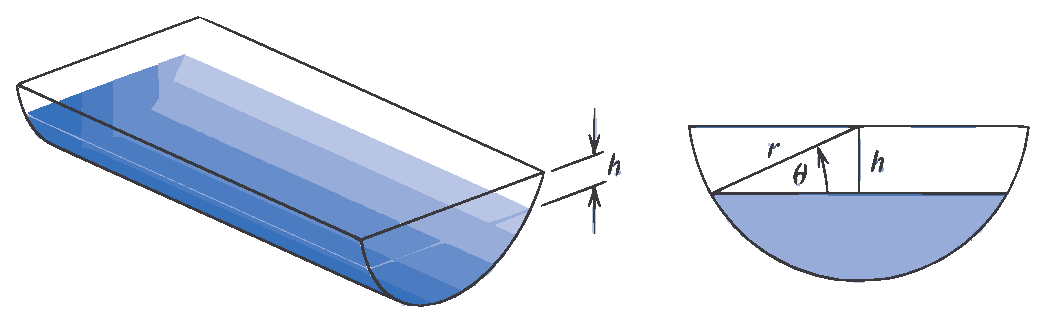
\includegraphics[scale=0.6]{img/tanque.eps}
\end{figure}

Suponga que $L=10\,ft$, $r=1\,ft$, y $V=12.4\,ft^3$. Encuentre la
\textbf{profundidad} del agua en el tanque con una tolerancia de $0.01\,ft$.
\begin{eqnarray} 
12.4 &=&10\,[0.5\,\pi\,1^2-1^2\,arcsin(h/1)-h\,(1^2-h^2)^{1/2}] \nonumber\\
12.4 &=&10\,[0.5\,\pi\,-arcsin(h)-h\,(1-h^2)^{1/2}] \nonumber
\end{eqnarray}

\par se necesita un $h$ tal que al sustituir en el miembro derecho de
$12.4$. Si se resta $12.4$ a la ecuación se tiene
\[
  0=10\,[0.5\,\pi\,-arcsin(h)-h\,(1-h^2)^{1/2}]-12.4
\]

\par luego se require un $h$, tal que al sustituir, de el valor de
$0$. En otras palabras, es menester hallar la raíz de la funcion, que
ahora lo definimos como $f\left(h\right)$
\[
  f\left(h\right)=10\,[0.5\,\pi\,-arcsin(h)-h\,(1-h^2)^{1/2}]-12.4=0
\]

\begin{verbatim}
  f(h):=10*(0.5*%pi-asin(h)-h*(1-h^2)^(1/2))-12.4;
  biseccion(0,1,3,20);
\end{verbatim}

$$\pmatrix{N&a&b&p&f\left(a\right)&f\left(b\right)&f\left(p\right)&f
 \left(a\right)\,f\left(p\right)&{\it error}\cr 1&0&1&0.5&3.30796&-
 12.4&-6.25815&-20.7017&0.5\cr 2&0&0.5&0.25&3.30796&-6.25815&-1.63945
 &-5.42325&0.25\cr 3&0&0.25&0.125&3.30796&-1.63945&0.8145&2.6943&
 0.125\cr 4&0.125&0.25&0.1875&0.8145&-1.63945&-0.4199&-0.342&0.0625
 \cr 5&0.125&0.1875&0.1563&0.8145&-0.4199&0.1957&0.1594&0.03125\cr 6&
 0.1563&0.1875&0.1719&0.1957&-0.4199&-0.1125&-0.02203&0.01563\cr 7&
 0.1563&0.1719&0.1641&0.1957&-0.1125&0.04149&0.008121&0.007813\cr 8&
 0.1641&0.1719&0.168&0.04149&-0.1125&-0.03555&-0.001475&0.003906\cr 9
 &0.1641&0.168&0.166&0.04149&-0.03555&0.002966&1.23086 \times 10^{-4}
 &0.001953\cr 10&0.166&0.168&0.167&0.002966&-0.03555&-0.01629&-
 4.832935 \times 10^{-5}&9.765625 \times 10^{-4}\cr }$$

por lo tanto $h=0.167$. Luego la profundidad es: radio menos el
valor de $h$ hallado
\[
  profundidad=r-h=1-0.167=0.833
\]

%%% Local Variables:
%%% TeX-master: "tarea1"
%%% End:


\chapter{Punto fijo\\
{\normalsize Ejercicios de Seccion 2.2, Pág. 64 }
}

\section{ejercicio 5}
Use iteraciones con el método de punto fijo y determine la solución de
$x^4-3\,x^2-3$ en el intervalo $[1,\,2]$ con una tolerancia de
$10^{-2}$.  Use $p_0=1$. Se escoge y verifica $g(x)$
$$
g(x)=\left(3\,x^2+3\right)^{1/4}\,; \quad
g\,'(x)={{1.5\,x}\over{\left(3\,x^2+3\right)^{0.75}}}\,; \quad
g\,'(1)=0.39127
$$

\begin{verbatim}
  g(x):=(3*x^2+3)^(1/4);
  puntofijo(1,2,20);
\end{verbatim}

\[
\pmatrix{N&x&g\left(x\right)&{\it error}\cr 1&1&1.5651&0.565\cr 2&
 1.5651&1.7936&0.228\cr 3&1.7936&1.8859&0.0924\cr 4&1.8859&1.9228&
 0.0369\cr 5&1.9228&1.9375&0.0147\cr 6&1.9375&1.9433&0.00581\cr }
\]

\section{ejercicio 11}
Determine el intervalo $[a,\,b]$ en el que las iteraciones de punto
fijo convergan. Estimar el numero de iteraciones necesarias para
obtener una aproximación con $10^{-5}$ de tolerancia. Obtenga la raiz.

\subsection{inciso b)}
$x=\frac{5}{x^2}+2$

\begin{verbatim}
  g(x):=5/x^2+2;
  puntofijo(2.6,5,20);
\end{verbatim}
\[
\pmatrix{N&x&g\left(x\right)&{\it error}\cr 1&2.6&2.739645&0.139645
 \cr 2&2.739645&2.6661644&0.0734806\cr 3&2.6661644&2.7033899&
 0.0372255\cr 4&2.7033899&2.684152&0.0192379\cr 5&2.684152&2.6939941&
 0.00984208\cr 6&2.6939941&2.6889326&0.00506153\cr 7&2.6889326&
 2.6915287&0.00259608\cr 8&2.6915287&2.6901953&0.00133336\cr 9&
 2.6901953&2.6908796&6.84344391 \times 10^{-4}\cr 10&2.6908796&
 2.6905283&3.5136427 \times 10^{-4}\cr 11&2.6905283&2.6907086&
 1.8036815 \times 10^{-4}\cr 12&2.6907086&2.690616&
 9.25984046 \times 10^{-5}\cr 13&2.690616&2.6906636&
 4.75363581 \times 10^{-5}\cr 14&2.6906636&2.6906392&
 2.44038989 \times 10^{-5}\cr 15&2.6906392&2.6906517&
 1.25281495 \times 10^{-5}\cr 16&2.6906517&2.6906453&
 6.4315776 \times 10^{-6}\cr }
\]

\subsection{inciso f)}
$x=0.5\,\left(\sin x+\cos x\right)$

\begin{verbatim}
  g(x):=0.5*(sin(x)+cos(x));
  puntofijo(0.6,5,20);
\end{verbatim}
\[
\pmatrix{N&x&g\left(x\right)&{\it error}\cr 1&0.6&0.694989&0.094989
 \cr 2&0.694989&0.704219&0.00922983\cr 3&0.704219&0.704778&
 5.59244952 \times 10^{-4}\cr 4&0.704778&0.70481&
 3.19565575 \times 10^{-5}\cr 5&0.70481&0.704812&
 1.81941422 \times 10^{-6}\cr }
\]

\section{ejercicio 13}
Encontrar los ceros de $f\left(x\right)=x^2+10\cos x$ usando el
método de punto fijo con la funcion iterativa $g$ apropiada. La
tolerancia es $10^{-4}$.

Primer cero en $x=-2.1$
$$
g(x)=-acos\left(\frac{-x^2}{10}\right)\,; \quad
g\,'(x)=-{{0.2\,x}\over{\left(1-0.01\,x^4\right)^{0.5}}}\,; \quad
g\,'(-2.1)=0.46796
$$


\begin{verbatim}
  g(x):=-acos((-x^2)/10);
  puntofijo(-2.1,4,20);
\end{verbatim}

\[
\pmatrix{N&x&g\left(x\right)&{\it error}\cr 1&-2.1&-2.027509&
 0.072491\cr 2&-2.027509&-1.994434&0.033075\cr 3&-1.994434&-1.979889&
 0.014545\cr 4&-1.979889&-1.973596&0.0062922\cr 5&-1.973596&-1.970894
 &0.0027025\cr 6&-1.970894&-1.969737&0.0011571\cr 7&-1.969737&-
 1.969242&4.9477865 \times 10^{-4}\cr 8&-1.969242&-1.969031&
 2.1144729 \times 10^{-4}\cr 9&-1.969031&-1.96894&
 9.034162 \times 10^{-5}\cr }
\]
otro cero en $x=1.8$

$$
g(x)=acos\left(\frac{-x^2}{10}\right)\,; \quad
g\,'(x)={{0.2\,x}\over{\left(1-0.01\,x^4\right)^{0.5}}}\,; \quad
g\,'(1.8)=0.46796
$$

\begin{verbatim}
g(x):=acos((-x^2)/10);
puntofijo(1.8,4,20);
\end{verbatim}
\[
\pmatrix{N&x&g\left(x\right)&{\it error}\cr 1&1.8&1.900751&0.10075
 \cr 2&1.900751&1.940442&0.039691\cr 3&1.940442&1.956846&0.016404\cr 
 4&1.956846&1.963756&0.0069106\cr 5&1.963756&1.966691&0.0029347\cr 6&
 1.966691&1.967942&0.0012505\cr 7&1.967942&1.968475&
 5.3360859 \times 10^{-4}\cr 8&1.968475&1.968703&
 2.2784079 \times 10^{-4}\cr 9&1.968703&1.9688&
 9.730918 \times 10^{-5}\cr }
\]

otro cero en $x=-3.2$ con un $g(x)$ diferente
$$
g(x)=\frac{2x^2-10cos(x)}{3x}\,; \quad
g\,'(x)={{0.33333\,\left(10\,x\,\sin x+10\,\cos x+2\,x^2\right)}\over{x^2}}\,; \quad
g\,'(-3.2)=0.28089
$$
\begin{verbatim}
g(x):=(2*x^2-10*cos(x))/(3*x);
puntofijo(-3.2,4,20);
\end{verbatim}

\[
\pmatrix{N&x&g\left(x\right)&{\it error}\cr 1&-3.2&-3.173224&
 0.026776\cr 2&-3.173224&-3.165413&0.0078103\cr 3&-3.165413&-3.163025
 &0.0023883\cr 4&-3.163025&-3.162285&7.4034559 \times 10^{-4}\cr 5&-
 3.162285&-3.162054&2.3046173 \times 10^{-4}\cr 6&-3.162054&-3.161983
 &7.183305 \times 10^{-5}\cr }
\]
otro cero en $x=3$

$$
g(x)=\frac{2x^2-10cos(x)}{3x}\,; \quad
g\,'(x)={{0.33333\,\left(10\,x\,\sin x+10\,\cos x+2\,x^2\right)}\over{x^2}}\,; \quad
g\,'(3)=0.4568
$$

\begin{verbatim}
puntofijo(3,4,20);
\end{verbatim}

\[
\pmatrix{N&x&g\left(x\right)&{\it error}\cr 1&3&3.099992&0.099992
 \cr 2&3.099992&3.141002&0.041011\cr 3&3.141002&3.155234&0.014231\cr 
 4&3.155234&3.159837&0.0046029\cr 5&3.159837&3.161289&0.0014524\cr 6&
 3.161289&3.161744&4.5464195 \times 10^{-4}\cr 7&3.161744&3.161886&
 1.4195461 \times 10^{-4}\cr 8&3.161886&3.16193&
 4.4287896 \times 10^{-5}\cr }
\]

\section{ejercicio 14}
Use el método punto fijo para determinar la solución, con una
tolerancia $10^{-4}$, de $x=tan(x)$, para $x$ en $[4,\,5]$. Para
hallar $g(x)$ se sigue
$$
\frac{1}{x}=\frac{1}{tan(x)}\,; \quad
0=\frac{1}{tan(x)}-\frac{1}{x}\,; \quad
x=\frac{1}{tan(x)}-\frac{1}{x}+x\,; \quad
luego \;\; x=g(x)=\frac{1}{tan(x)}-\frac{1}{x}+x
$$
probando $g(x)$
$$
g\,'(x)=-{{\sec ^2x}\over{\tan ^2x}}+{{1}\over{x^2}}+1\,; \quad
g\,'(4)=- 0.68346
$$
\begin{verbatim}
g(x):=1/tan(x)-1/x+x;
puntofijo(4,4,20);
\end{verbatim}

\[
\pmatrix{N&x&g\left(x\right)&{\it error}\cr 1&4&4.613691&0.61369
 \cr 2&4.613691&4.495965&0.11773\cr 3&4.495965&4.493411&0.0025536\cr 
 4&4.493411&4.493409&1.4462156 \times 10^{-6}\cr }
\]

%%% Local Variables:
%%% TeX-master: "tarea1"
%%% End:

\chapter{Newton, Secante y Posicion falsa\\
{\normalsize Ejercicios de Seccion 2.3, Pág. 75 }
}
\section{ejercicio 1}
Sea $f(x)=x^2-6$ y $p_0=1$. Use el método de Newton para encontrar $p_2$.
$$
f\,'(x)=2\,x
$$
\begin{verbatim}
f(x):=x^2-6;
newton(1,4,2);
\end{verbatim}
$$
\pmatrix{
N& X_n& X_{n+1}&error\cr 
1&1&3.5&2.5\cr 
2&3.5&2.607143&0.89286\cr 
}
$$

\section{ejercicio 3}
Sea $f(x)=x^2-6$. Con $p_0=3$ y $p_1=2$, buscar $p_3$.

\subsection{inciso a)}
Usando el método de la secante.
\begin{verbatim}
f(x):=x^2-6;
secante(3,2,4,3);
\end{verbatim}

$$\pmatrix{N& X_{n-1}& X_n&X_{n+1}& error\cr 1&3&
 2&2.4&0.4\cr 2&2&2.4&2.454545&0.054545\cr 3&2.4&2.454545&2.449438&
 0.0051073\cr }$$

\subsection{inciso b)}
Usando el método de posicion falsa.
\begin{verbatim}
posicionfalsa(3,2,4,3);
\end{verbatim}
$$\pmatrix{N&X_{n-1}&X_n&X_{n+1}&error\cr 1&3&
 2&2.4&0.4\cr 2&3&2.4&2.444444&0.044444\cr 3&3&2.444444&2.44898&
 0.0045351\cr }$$

\subsection{inciso c)}
El inciso a) o el inciso b) está mas cerca de $\sqrt{6}\,$?\\

R// Por el método de la secante $p_3=2.449438$  y por el método de 
posición falsa $p_3=2.44898$. Dado que $\sqrt{6}=2.4494897427$ decimos
que el inciso a) por el método de la secante es más exacto.

\section{ejercicio 5}
Use el método de Newton para encontrar la solucion con una tolerancia $10^{-4}$ 
para los siguientes problemas.
\subsection{inciso a)}
Para $f(x)=x^3-2x^2-5=0$ en el intervalo $[1,\,4]$.
$$
  f\,'(x)=3\,x^2-4\,x
$$
\begin{verbatim}
f(x):=x^3-2*x^2-5;
newton(2.5,4,20);
\end{verbatim}

$$\pmatrix{N&X_n&X_{n+1}& error\cr 1&2.5&2.714286&
 0.21429\cr 2&2.714286&2.690952&0.023334\cr 3&2.690952&2.690647&
 3.0401747 \times 10^{-4}\cr 4&2.690647&2.690647&
 5.1228279 \times 10^{-8}\cr }$$

\subsection{inciso c)}
Para $f(x)=x-cos(x)=0$ en el intervalo $[0,\,\pi/2]$.
$$
f\,'(x)=sin(x)+1
$$

\begin{verbatim}
f(x):=x-cos(x);
newton(0,4,20);
\end{verbatim}

$$\pmatrix{N&X_n&X_{n+1}& error\cr 1&0&1.0&1.0\cr 2&
 1.0&0.75036&0.24964\cr 3&0.75036&0.73911&0.011251\cr 4&0.73911&
 0.73909&2.7757526 \times 10^{-5}\cr }$$

\section{ejercicio 6}
Use el método de Newton para encontrar la solución con una tolerancia $10^{-5}$
para los siguientes problemas
\subsection{inciso b)}
Para $f(x)=ln(x-1)+cos(x-1)=0$ en el intervalo $[1.3,\,2]$
$$
f\,'(x)={{1.0}\over{x-1}}-\sin \left(x-1\right)
$$

\begin{verbatim}
f(x):=ln(x-1)+cos(x-1);
newton(1.3, 5, 20);
\end{verbatim}

$$\pmatrix{N& X_n& X_{n+1}&error\cr 1&1.3&1.3818471&
 0.0818471\cr 2&1.3818471&1.3973207&0.0154736\cr 3&1.3973207&
 1.3977482&4.27431534 \times 10^{-4}\cr 4&1.3977482&1.3977485&
 3.1148496 \times 10^{-7}\cr }$$

\subsection{inciso e)}
Para $f(x)=e^x-3x^2=0$ en el intervalo $[0,\,1]$ y $[3,\,5]$.
$$
f\,'(x)=e^{x}-6\,x
$$

\subsubsection{intervalo[0, 1]}
$$
f\,'(x)=e^{x}-6\,x
$$

\begin{verbatim}
f(x):=%e^x-3*x^2;
newton(0.5, 5, 20);
\end{verbatim}

$$\pmatrix{N&X_n&X_{n+1}& error\cr 1&0.5&1.1650895&
 0.665089\cr 2&1.1650895&0.936227&0.228863\cr 3&0.936227&0.910397&
 0.0258303\cr 4&0.910397&0.910008&3.89003009 \times 10^{-4}\cr 5&
 0.910008&0.910008&8.93744134 \times 10^{-8}\cr }$$

\subsubsection{intervalo[3,5]}
$$
f\,'(x)=e^{x}-6\,x
$$

\begin{verbatim}
f(x):=%e^x-3*x^2;
newton(3, 5, 20);
\end{verbatim}

$$\pmatrix{N&X_n&X_{n+1}& error\cr 1&3&6.3154355&
 3.3154355\cr 2&6.3154355&5.4741495&0.841286\cr 3&5.4741495&4.7516461
 &0.722503\cr 4&4.7516461&4.2011347&0.550511\cr 5&4.2011347&3.868723&
 0.332412\cr 6&3.868723&3.7479169&0.120806\cr 7&3.7479169&3.733279&
 0.0146379\cr 8&3.733279&3.7330791&1.99887999 \times 10^{-4}\cr 9&
 3.7330791&3.733079&3.68620818 \times 10^{-8}\cr }$$

\section{ejercicio 7}
Utilice el método de la secante para encontrar la solución, con una tolerancia
$10^{-4}$, para los siguientes problemas.

\subsection{inciso b)}
Para $f(x)=x^3+3x^2-1=0$ en el intervalo $[-3,\,-2]$.
\begin{verbatim}
f(x):=x^3+3*x^2-1;
secante(-3, -2, 4, 20);
\end{verbatim}

$$\pmatrix{N&X_{n-1}&X_n&X_{n+1}& error\cr 1&-3
 &-2&-2.75&0.75\cr 2&-2&-2.75&-3.066667&0.31667\cr 3&-2.75&-3.066667&
 -2.862024&0.20464\cr 4&-3.066667&-2.862024&-2.877186&0.015162\cr 5&-
 2.862024&-2.877186&-2.879414&0.002228\cr 6&-2.877186&-2.879414&-
 2.879385&2.870283 \times 10^{-5}\cr }$$

\subsection{inciso d)}
Para $f(x)=x-0.8-0.2sin(x)=0$ en el intervalo $[0,\,\pi/2]$

\begin{verbatim}
f(x):=x-0.8-0.2*sin(x);
secante(0, %pi/2, 4, 20);
\end{verbatim}

$$\pmatrix{N& X_{n-1}&X_n&X_{n+1}&error\cr 1&0&
 1.570796&0.91672&0.65408\cr 2&1.570796&0.91672&0.96155&0.044831\cr 3
 &0.91672&0.96155&0.96435&0.0027948\cr 4&0.96155&0.96435&0.96433&
 1.2200555 \times 10^{-5}\cr }$$

\section{ejercicio 9}
Utilice el método de posicion falsa para encontrar la solución, con
una tolerancia $10^{-4}$, para los siguientes problemas.

\subsection{inciso b)}
Para $f(x)=x^3+3x^2-1=0$ en el intervalo $[-3,\,-2]$.
\begin{verbatim}
f(x):=x^3+3*x^2-1;
posicionfalsa(-3, -2, 4, 20);
\end{verbatim}

$$\pmatrix{N& X_{n-1}& X_n&X_{n+1}& error\cr 1&-3
 &-2&-2.75&0.75\cr 2&-3&-2.75&-2.867769&0.11777\cr 3&-3&-2.867769&-
 2.878406&0.010638\cr 4&-3&-2.878406&-2.879303&
 8.9706978 \times 10^{-4}\cr 5&-3&-2.879303&-2.879378&
 7.5196398 \times 10^{-5}\cr }$$


\subsection{inciso d)}
Para $f(x)=x-0.8-0.2sin(x)=0$ en el intervalo $[0,\,\pi/2]$

\begin{verbatim}
f(x):=x-0.8-0.2*sin(x);
posicionfalsa(0, %pi/2, 4, 20);
\end{verbatim}

$$\pmatrix{N& X_{n-1}&X_n&X_{n+1}& error \cr 1&0&
 1.570796&0.91672&0.65408\cr 2&0.91672&1.570796&0.96155&0.044831\cr 3
 &0.96155&1.570796&0.96417&0.0026194\cr 4&0.96417&1.570796&0.96432&
 1.5355164 \times 10^{-4}\cr 5&0.96432&1.570796&0.96433&
 9.0027664 \times 10^{-6}\cr }$$

\section{ejercicio 11}
Use los tres métodos (newton, secante y posicion falsa) para buscar la
soluncion, con una tolerancia $10^{-5}$, para los siguientes problemas.

\subsection{inciso a)}
Para $f(x)=3xe^x=0$ en el intervalo $[1,\,2]$.

\subsubsection{Newton}
$$
f\,'(x)=3\,x\,e^{x}+3\,e^{x}
$$
\begin{verbatim}
f(x):=3*x*%e^x;
newton(1.3, 5, 20);
\end{verbatim}

$$\pmatrix{N& X_n&X_{n+1}& error\cr 1&1.3&0.734783&
 0.565217\cr 2&0.734783&0.311224&0.423559\cr 3&0.311224&0.0738701&
 0.237354\cr 4&0.0738701&0.00508142&0.0687887\cr 5&0.00508142&
 2.569032 \times 10^{-5}&0.00505573\cr 6&2.569032 \times 10^{-5}&
 6.59975587 \times 10^{-10}&2.568966 \times 10^{-5}\cr 7&
 6.59975587 \times 10^{-10}&4.35567771 \times 10^{-19}&
 6.59975586 \times 10^{-10}\cr }$$

\subsubsection{Secante}
\begin{verbatim}
f(x):=3*x*%e^x;
secante(1, 2, 5, 20);
\end{verbatim}

$$\pmatrix{N& X_{n-1}& X_n&X_{n+1}& error\cr 1&1&
 2&0.7746&1.2253997\cr 2&2&0.7746&0.617357&0.157244\cr 3&0.7746&
 0.617357&0.281622&0.335735\cr 4&0.617357&0.281622&0.119176&0.162446
 \cr 5&0.281622&0.119176&0.0279083&0.0912673\cr 6&0.119176&0.0279083&
 0.00309614&0.0248122\cr 7&0.0279083&0.00309614&
 8.50847825 \times 10^{-5}&0.00301106\cr 8&0.00309614&
 8.50847825 \times 10^{-5}&2.63016187 \times 10^{-7}&
 8.48217663 \times 10^{-5}\cr 9&8.50847825 \times 10^{-5}&
 2.63016187 \times 10^{-7}&2.23777201 \times 10^{-11}&
 2.6299381 \times 10^{-7}\cr }$$

\subsubsection{Posicion falsa}
\begin{verbatim}
f(x):=3*x*%e^x;
posicionfalsa(1, 2, 5, 20);
\end{verbatim}

$$\pmatrix{N& X_{n-1}& X_n& X_{n+1}& error\cr 1&1&
 2&0.7746&1.2254\cr 2&1&0.7746&0.4095&0.3651\cr 3&1&0.4095&0.2362&
 0.1733\cr 4&1&0.2362&0.1418&0.09445\cr 5&1&0.1418&0.08689&0.05487
 \cr 6&1&0.08689&0.0539&0.03299\cr 7&1&0.0539&0.03368&0.02022\cr 8&1&
 0.03368&0.02114&0.01254\cr 9&1&0.02114&0.0133&0.007836\cr 10&1&
 0.0133&0.008383&0.004917\cr 11&1&0.008383&0.00529&0.003094\cr 12&1&
 0.00529&0.00334&0.00195\cr 13&1&0.00334&0.00211&0.00123\cr 14&1&
 0.00211&0.001333&7.767375 \times 10^{-4}\cr }$$

\subsection{inciso b)}
Para $f(x)=2\,x+3\,cos(x)-e^x=0$ en el intervalo $[0,\,1]$.

$$
f\,'(x)=-3\,\sin x-e^{x}+2
$$
\subsubsection{Newton}
\begin{verbatim}
f(x):=2*x+3*cos(x)-%e^x;
newton(0.5, 5, 20);
\end{verbatim}

$$\pmatrix{N& X_n& X_{n+1}&error\cr 1&0.5&2.3252348&
 1.8252348\cr 2&2.3252348&1.592329&0.732906\cr 3&1.592329&1.288817&
 0.303512\cr 4&1.288817&1.2409046&0.0479124\cr 5&1.2409046&1.2397154&
 0.00118917\cr 6&1.2397154&1.2397147&7.29899547 \times 10^{-7}\cr }$$

\subsubsection{Secante}
\begin{verbatim}
f(x):=2*x+3*cos(x)-%e^x;
secante(0.5, 1, 5, 20);
\end{verbatim}

$$\pmatrix{N& X_{n-1}&X_n& X_{n+1}& error\cr 1&
 0.5&1&1.4173405&0.41734\cr 2&1&1.4173405&1.217055&0.200285\cr 3&
 1.4173405&1.217055&1.2377761&0.0207211\cr 4&1.217055&1.2377761&
 1.2397376&0.0019615\cr 5&1.2377761&1.2397376&1.2397147&
 2.29590039 \times 10^{-5}\cr 6&1.2397376&1.2397147&1.2397147&
 2.29674058 \times 10^{-8}\cr }$$

\subsubsection{Posicion falsa}
\begin{verbatim}
f(x):=2*x+3*cos(x)-%e^x;
posicionfalsa(0.5, 1, 5, 20);
\end{verbatim}

$$\pmatrix{N& X_{n-1}& X_n&X_{n+1}&error\cr 1&
 0.5&1&1.4173405&0.41734\cr 2&1.4173405&1&1.217055&0.200285\cr 3&
 1.217055&1.4173405&1.2377761&0.0207211\cr 4&1.2377761&1.4173405&
 1.2395503&0.00177417\cr 5&1.2395503&1.4173405&1.2397008&
 1.5046154 \times 10^{-4}\cr 6&1.2397008&1.4173405&1.2397135&
 1.27497504 \times 10^{-5}\cr 7&1.2397135&1.4173405&1.2397146&
 1.08030887 \times 10^{-6}\cr }$$

\section{ejercicio 17}
El polinomio de cuarto grado 
$$
f(x)=230\,x^4+18\,x^3+9\,x^2-221\,x-9
$$
tiene dos ceros reales, la una en $[-1,\,0]$ y la otra en $[0,\,1]$.
Aproximar estos ceros con $10^{-6}$ usando:

\begin{itemize}
\item Método de Posicion falsa
\item Método de la Secante
\item Método de Newton
\end{itemize}

\subsection{inciso a)}

\subsubsection{intervalo [-1, 0]}

\begin{verbatim}
f(x):=230*x^4+18*x^3+9*x^2-221*x-9;
posicionfalsa(-1, 0, 6, 30);
\end{verbatim}

$$\pmatrix{N& X_{n-1}& X_n&X_{n+1}& error\cr 1&-1
 &0&-0.02036199&0.02036199\cr 2&-1&-0.02036199&-0.03043025&0.01006826
 \cr 3&-1&-0.03043025&-0.03547981&0.005049567\cr 4&-1&-0.03547981&-
 0.03803041&0.002550599\cr 5&-1&-0.03803041&-0.03932338&0.001292966
 \cr 6&-1&-0.03932338&-0.03998001&6.566287334 \times 10^{-4}\cr 7&-1&
 -0.03998001&-0.04031378&3.337740601 \times 10^{-4}\cr 8&-1&-
 0.04031378&-0.04048352&1.697416654 \times 10^{-4}\cr 9&-1&-
 0.04048352&-0.04056987&8.634310068 \times 10^{-5}\cr 10&-1&-
 0.04056987&-0.04061379&4.392576813 \times 10^{-5}\cr 11&-1&-
 0.04061379&-0.04063614&2.23479565 \times 10^{-5}\cr 12&-1&-
 0.04063614&-0.04064751&1.137024619 \times 10^{-5}\cr 13&-1&-
 0.04064751&-0.0406533&5.785072919 \times 10^{-6}\cr 14&-1&-0.0406533
 &-0.04065624&2.943413834 \times 10^{-6}\cr 15&-1&-0.04065624&-
 0.04065774&1.497599226 \times 10^{-6}\cr 16&-1&-0.04065774&-
 0.0406585&7.61975133 \times 10^{-7}\cr }$$

\subsubsection{intervalo [0, 1]}

\begin{verbatim}
f(x):=230*x^4+18*x^3+9*x^2-221*x-9;
posicionfalsa(0, 1, 6, 30);
\end{verbatim}

$$\pmatrix{N& X_{n-1}& X_n& X_{n+1}& error\cr 1&0&
 1&0.25&0.75\cr 2&0.25&1&0.7737628&0.5237628\cr 3&0.7737628&1&
 0.9448852&0.1711224\cr 4&0.9448852&1&0.9611108&0.01622563\cr 5&
 0.9611108&1&0.9623057&0.001194866\cr 6&0.9623057&1&0.9623917&
 8.608441294 \times 10^{-5}\cr 7&0.9623917&1&0.9623979&
 6.1920579 \times 10^{-6}\cr 8&0.9623979&1&0.9623984&
 4.453438442 \times 10^{-7}\cr }$$

\subsection{inciso b)}

\subsubsection{intervalo [-1, 0]}

\begin{verbatim}
f(x):=230*x^4+18*x^3+9*x^2-221*x-9;
secante(-1, 0, 6, 30);
\end{verbatim}

$$\pmatrix{N& X_{n-1}& X_n& X_{n+1}& error\cr 1&-1
 &0&-0.02036199&0.02036199\cr 2&0&-0.02036199&-0.04069126&0.02032927
 \cr 3&-0.02036199&-0.04069126&-0.04065926&3.199385755 \times 10^{-5}
 \cr 4&-0.04069126&-0.04065926&-0.04065929&2.573803404 \times 10^{-8}
 \cr }$$

\subsubsection{intervalo [1,0]}
\begin{verbatim}
f(x):=230*x^4+18*x^3+9*x^2-221*x-9;
secante(0.5, 1, 6, 30);
\end{verbatim}

$$\pmatrix{N& X_{n-1}& X_n& X_{n+1}& error\cr 1&
 0.5&1&0.8942214&0.1057786\cr 2&1&0.8942214&0.9570464&0.062825\cr 3&
 0.8942214&0.9570464&0.9632104&0.006164091\cr 4&0.9570464&0.9632104&
 0.9623896&8.208126831 \times 10^{-4}\cr 5&0.9632104&0.9623896&
 0.9623984&8.772062474 \times 10^{-6}\cr 6&0.9623896&0.9623984&
 0.9623984&1.432207719 \times 10^{-8}\cr }$$

\subsection{inciso c)}

\subsubsection{intervalo [-1, 0]}
$$
f\,'(x)=920\,x^3+54\,x^2+18\,x-221
$$
\begin{verbatim}
f(x):=230*x^4+18*x^3+9*x^2-221*x-9;
newton(-0.5, 6, 30);
\end{verbatim}

$$\pmatrix{N& X_n& X_{n+1}& error\cr 1&-0.5&-0.1504525
 &0.3495475\cr 2&-0.1504525&-0.04181681&0.1086357\cr 3&-0.04181681&-
 0.04065934&0.00115747\cr 4&-0.04065934&-0.04065929&
 5.518157035 \times 10^{-8}\cr }$$

\subsubsection{intervalo [0, 1]}
$$
f\,'(x)=920\,x^3+54\,x^2+18\,x-221
$$

\begin{verbatim}
f(x):=230*x^4+18*x^3+9*x^2-221*x-9;
newton(0.7, 6, 30);
\end{verbatim}

$$\pmatrix{N& X_n& X_{n+1}& error\cr 1&0.7&1.43262236&
 0.7326224\cr 2&1.43262236&1.15993576&0.2726866\cr 3&1.15993576&
 1.01378674&0.146149\cr 4&1.01378674&0.9670653&0.04672145\cr 5&
 0.9670653&0.9624416&0.004623643\cr 6&0.9624416&0.9623984&
 4.322351778 \times 10^{-5}\cr 7&0.9623984&0.9623984&
 3.754473843 \times 10^{-9}\cr }$$

\section{ejercicio 24}
Buscar una aproximación de $\lambda{}$, con $10^{-4}$, para la siguiente ecuación
$$
1564000=1000000\,e^{\lambda}+\frac{435000}{\lambda} \left(e^{\lambda}-1\right)
$$

$$
f\,'(x)={{435000\,e^{x}}\over{x}}+1000000\,e^{x}-{{435000\,\left(e^{x}-1
 \right)}\over{x^2}}
$$

\begin{verbatim}
f(x):=1000000*%e^x+435000/x*(%e^x-1)-1564000;
newton(0.01, 4, 20);
\end{verbatim}

$$\pmatrix{N&X_n& X_{n+1}& error\cr 1&0.01&0.10501&
 0.09501\cr 2&0.10501&0.10101&0.0040043\cr 3&0.10101&0.101&
 7.5800338 \times 10^{-6}\cr }$$

\section{ejercicio 25}
La suma de dos numeros da 20. Si a ámbos se les añade su raiz cuadrada
y se multiplican da 155.55.
$$
x+y=20 \quad \longrightarrow \quad y=20-x
$$
\begin{eqnarray}
\left(x+\sqrt{x}\right)\left(y+\sqrt{y}\right)&=&155.55 \nonumber\\
\left(x+\sqrt{x}\,\right)\left(20-x+\sqrt{20-x} \, \right)&=&155.55 \nonumber\\
\left(x+\sqrt{x}\,\right)\left(20-x+\sqrt{20-x} \, \right)-155.55&=&0=f(x) \nonumber
\end{eqnarray}
\begin{verbatim}
f(x):=(x+sqrt(x))*(20-x+sqrt(20-x))-155.55;
secante(6, 7, 6, 20);
\end{verbatim}

$$\pmatrix{N& X_{n-1}&X_n& X_{n+1}& error\cr 1&6&
 7&6.54963582&0.4503642\cr 2&7&6.54963582&6.50999293&0.03964289\cr 3&
 6.54963582&6.50999293&6.51286432&0.002871395\cr 4&6.50999293&
 6.51286432&6.51284873&1.559160583 \times 10^{-5}\cr 5&6.51286432&
 6.51284873&6.51284873&6.580253675 \times 10^{-9}\cr }$$

\begin{verbatim}
f(x):=(x+sqrt(x))*(20-x+sqrt(20-x))-155.55;
secante(13, 14, 6, 20);
\end{verbatim}

$$\pmatrix{N& X_{n-1}& X_n&X_{n+1}& error\cr 1&13
 &14&13.4503642&0.5496358\cr 2&14&13.4503642&13.4845347&0.03417049
 \cr 3&13.4503642&13.4845347&13.4871656&0.002630904\cr 4&13.4845347&
 13.4871656&13.4871513&1.430811379 \times 10^{-5}\cr 5&13.4871656&
 13.4871513&13.4871513&5.532454495 \times 10^{-9}\cr }$$

por lo tanto los dos numeros son: $x=6.512849$ y $y=13.487151$

%%% Local Variables:
%%% TeX-master: "tarea1"
%%% End:

\chapter{Newton\\
{\normalsize Ejercicios de Seccion 2.4, Pág. 85 }
}
\section{ejercicio 1}
Use el método de newton para encontrar la solución, con $10^{-5}$, para
los siguientes problemas.

\subsection{inciso a)}
Con $x^2-2\,x\,e^{-x}+e^{-2x}=0$, para $0 \leq x \leq 1$

$$f\,'(x)=2\,x\,e^ {- x }-2\,e^ {- x }-2\,e^ {- 2\,x }+2\,x$$

\begin{verbatim}
f(x):=x^2-2*x*%e^(-x)+%e^(-2*x);
newton(0.4, 5, 20);
\end{verbatim}

$$\pmatrix{N&X_n& X_{n+1}& error\cr 1&0.4&0.480919&
 0.0809186\cr 2&0.480919&0.523341&0.0424222\cr 3&0.523341&0.545066&
 0.0217253\cr 4&0.545066&0.55606&0.0109942\cr 5&0.55606&0.561591&
 0.00553032\cr 6&0.561591&0.564364&0.00277352\cr 7&0.564364&0.565753&
 0.00138885\cr 8&0.565753&0.566448&6.949512 \times 10^{-4}\cr 9&
 0.566448&0.566796&3.47606794 \times 10^{-4}\cr 10&0.566796&0.566969&
 1.73836207 \times 10^{-4}\cr 11&0.566969&0.567056&
 8.69263072 \times 10^{-5}\cr 12&0.567056&0.5671&
 4.34652049 \times 10^{-5}\cr 13&0.5671&0.567122&
 2.17331155 \times 10^{-5}\cr 14&0.567122&0.567132&
 1.08666849 \times 10^{-5}\cr 15&0.567132&0.567138&
 5.43337546 \times 10^{-6}\cr }$$

\subsection{inciso d)}
con $f(x)=e^{6x}+3(ln\,2)^2\,e^{2x}-(ln\,8)e^{4x}-(ln\,2)^3=0$ para $-1 \leq x \leq 0$

$$f\,'(x)=6\,e^{6\,x}-8.3177662\,e^{4\,x}+2.8827181\,e^{2\,x}$$

\begin{verbatim}
f(x):=%e^(6*x)+3*(ln(2))^2*%e^(2*x)-(ln(8))^(4*x)-(ln(2))^3;
newton(-0.226, 5, 20);
\end{verbatim}

$$\pmatrix{N& X_n&X_{n+1}& error\cr 1&-0.226&-
 0.211125&0.0148746\cr 2&-0.211125&-0.201572&0.00955342\cr 3&-
 0.201572&-0.195354&0.00621838\cr 4&-0.195354&-0.191272&0.00408156
 \cr 5&-0.191272&-0.188579&0.0026934\cr 6&-0.188579&-0.186795&
 0.00178354\cr 7&-0.186795&-0.185611&0.00118374\cr 8&-0.185611&-
 0.184825&7.86825148 \times 10^{-4}\cr 9&-0.184825&-0.184301&
 5.23519142 \times 10^{-4}\cr 10&-0.184301&-0.183952&
 3.48556248 \times 10^{-4}\cr 11&-0.183952&-0.18372&
 2.32168422 \times 10^{-4}\cr 12&-0.18372&-0.183566&
 1.54689109 \times 10^{-4}\cr 13&-0.183566&-0.183463&
 1.03086573 \times 10^{-4}\cr 14&-0.183463&-0.183394&
 6.87065421 \times 10^{-5}\cr 15&-0.183394&-0.183348&
 4.57965054 \times 10^{-5}\cr 16&-0.183348&-0.183318&
 3.05275326 \times 10^{-5}\cr 17&-0.183318&-0.183297&
 2.03511819 \times 10^{-5}\cr 18&-0.183297&-0.183284&
 1.35694578 \times 10^{-5}\cr 19&-0.183284&-0.183275&
 9.05340675 \times 10^{-6}\cr }$$

\section{ejercicio 2}
Use el método de newton para encontrar la solución, con $10^{-5}$, para
los siguientes problemas.

\subsection{inciso b)}
Con $f(x)=x^2+6x^5+9x^4-2x^3-6x^2+1=0$ para $-3 \leq x  \leq -2$

$$f\,'(x)=30\,x^4+36\,x^3-6\,x^2-10\,x$$

\begin{verbatim}
f(x):=x^2+6*x^5+9*x^4-2*x^3-6*x^2+1;
newton(-2, 5, 20);
\end{verbatim}

$$\pmatrix{N& X_n& X_{n+1}& error\cr 1&-2&-1.7287234&
 0.271277\cr 2&-1.7287234&-1.5335706&0.195153\cr 3&-1.5335706&-
 1.4086994&0.124871\cr 4&-1.4086994&-1.3490539&0.0596455\cr 5&-
 1.3490539&-1.3350657&0.0139882\cr 6&-1.3350657&-1.3343478&
 7.17972296 \times 10^{-4}\cr 7&-1.3343478&-1.3343459&
 1.8315956 \times 10^{-6}\cr }$$

\subsection{inciso d)}
con $f(x)=e^{3x}-27\,x^6+27\,x^4\,e^x-9x^2e^{2x}=0$ para $3 \leq x  \leq 5$

$$f\,'(x)=3\,e^{3\,x}-18\,x^2\,e^{2\,x}-18\,x\,e^{2\,x}+27\,x^4\,e^{x}+108\,x
 ^3\,e^{x}-162\,x^5$$


\begin{verbatim}
f(x):=%e^(3*x)-27*x^6+27*x^4*%e^x-9*x^2*%e^(2*x);
newton(3.75 , 5, 20);
\end{verbatim}

$$\pmatrix{N& X_n& X_{n+1}&error\cr 1&3.75&3.7444462&
 0.00555385\cr 2&3.7444462&3.7406964&0.00374979\cr 3&3.7406964&
 3.738175&0.00252142\cr 4&3.738175&3.7364843&0.0016907\cr 5&3.7364843
 &3.7353527&0.00113152\cr 6&3.7353527&3.7345964&
 7.56314696 \times 10^{-4}\cr 7&3.7345964&3.7340913&
 5.05089051 \times 10^{-4}\cr 8&3.7340913&3.7337542&
 3.37114627 \times 10^{-4}\cr 9&3.7337542&3.7335293&
 2.24917153 \times 10^{-4}\cr 10&3.7335293&3.7333793&
 1.50029691 \times 10^{-4}\cr 11&3.7333793&3.7332792&
 1.00038024 \times 10^{-4}\cr 12&3.7332792&3.7332125&
 6.67225522 \times 10^{-5}\cr 13&3.7332125&3.7331678&
 4.46622606 \times 10^{-5}\cr 14&3.7331678&3.7331384&
 2.94270173 \times 10^{-5}\cr 15&3.7331384&3.73312&
 1.84303995 \times 10^{-5}\cr 16&3.73312&3.733105&
 1.50264624 \times 10^{-5}\cr 17&3.733105&3.7330931&
 1.18391299 \times 10^{-5}\cr 18&3.7330931&3.7330998&
 6.68252653 \times 10^{-6}\cr }$$

\section{ejercicio 5}
Use el método de newton y para encontrar la solución, con $10^{-5}$ para
$$
f(x)=e^{6x}+1.441e^{2x}-2.079e^{4x}-0.3330=0,\quad \quad para \quad -1 \leq x \leq 0
$$

$$f\,'(x)=6\,e^{6\,x}-8.316\,e^{4\,x}+2.882\,e^{2\,x}$$

\begin{verbatim}
f(x):=%e^(6*x)+1.441*%e^(2*x)-2.079*%e^(4*x)-0.3330;
newton(-0.16, 5, 20);
\end{verbatim}

$$\pmatrix{N& X_n& X_{n+1}& error\cr 1&-0.16&-0.166343
 &0.00634307\cr 2&-0.166343&-0.16908&0.00273704\cr 3&-0.16908&-
 0.16959&5.10103882 \times 10^{-4}\cr 4&-0.16959&-0.169607&
 1.63192092 \times 10^{-5}\cr 5&-0.169607&-0.169607&
 1.62934153 \times 10^{-8}\cr }$$



%%% Local Variables:
%%% TeX-master: "tarea1"
%%% End:


\chapter{Steffensen\\
{\normalsize Ejercicios de Seccion 2.5, Pág. 90 }
}
% pagina 90, seccion 2.5
\section{ejercicio 4}
Sea \(g(x)=1+(sin\,x)^2\) y \(p_0=1\). Use el método de steffensen
para encontrar \(p_{n+2}^{(1)}\) y \(p_{n+2}^{(2)}\)

\begin{verbatim}
g(x):=1+(sin(x))^2;
steffensen(1, 4, 20);
\end{verbatim}


$$\pmatrix{k & p_0^{(k)} & p_1^{(k)} & p_2^{(k)} & p_{n+2} & error\cr 1&1&1.708073&1.981273&2.152905&
 1.152905\cr 2&2.152905&1.697735&1.983973&1.873464&0.27944\cr }$$

por lo tanto \(p_{n+2}^{(1)}=2.152905\) y \(p_{n+2}^{(2)}=1.873464\)

\section{ejercicio 8}
Use el método de steffensen para encontrar, con una tolerancia menor a
$10^{-4}$, la raiz de $x-2^{-x}=0$ en el intervalo $[0,\,1]$

\begin{verbatim}
g(x):=2^(-x);
steffensen(0,4,20);
\end{verbatim}

$$\pmatrix{k & p_0^{(k)} & p_1^{(k)} & p_2^{(k)} & p_{n+2} & error\cr 1&0&1&0.5&0.66667&0.66667\cr 2&
 0.66667&0.62996&0.64619&0.64122&0.02545\cr 3&0.64122&0.64117&0.64119
 &0.64119&3.0447173 \times 10^{-5}\cr }$$

por lo tanto la solución aproximada es 0.64119

\section{ejercicio 9}
Use el método de steffensen con $p_0=2$ y calcule una aproximación de
$\sqrt{3}$ con una tolerancia $10^{-4}$.

\begin{verbatim}
g(x):=0.5*(x+3/x);
steffensen(2, 4, 20);
\end{verbatim}

$$\pmatrix{k & p_0^{(k)} & p_1^{(k)} & p_2^{(k)} & p_{n+2} & error\cr 1&2&1.75&1.732143&1.730769&0.26923
 \cr 2&1.730769&1.732051&1.732051&1.732051&0.0012816\cr 3&1.732051&
 1.732051&1.732051&1.732051&1.756042 \times 10^{-10}\cr }$$

por la aproximación a $\sqrt{3}$ es $1.732051$

\section{ejercicio 12}

\subsection{inciso b)}

Use el método de steffensen para aproximar la solución de $x^3-2x-5=0$
con una toleracia menor a $10^{-5}$. Use $g(x)=\sqrt[3]{2x+5}$.

\begin{verbatim}
g(x):=(2*x+5)^(1/3);
steffensen(1, 5, 20);
\end{verbatim}

$$\pmatrix{k & p_0^{(k)} & p_1^{(k)} & p_2^{(k)} & p_{n+2} & error\cr 1&1&1.9129312&2.0665808&2.0976736&
 1.0976736\cr 2&2.0976736&2.0950258&2.0946236&2.0945515&0.00312207
 \cr 3&2.0945515&2.0945515&2.0945515&2.0945515&
 1.92422669 \times 10^{-8}\cr }$$

por lo tanto la aproximación a la solucion es $2.0945515$

\subsection{inciso c)}

Use el método de steffensen para aproximar la solución de $3\,x^2-e^x=0$
con una toleracia menor a $10^{-5}$. Use $g(x)=\sqrt{\frac{e^x}{3}}$.

\begin{verbatim}
g(x):=sqrt((%e^x)/(3));
steffensen(0, 5, 20);
\end{verbatim}

$$\pmatrix{k & p_0^{(k)} & p_1^{(k)} & p_2^{(k)} & p_{n+2} & error\cr 1&0&0.57735&0.770565&0.86775&
 0.86775\cr 2&0.86775&0.890982&0.901392&0.909844&0.0420938\cr 3&
 0.909844&0.909933&0.909974&0.910008&1.64019988 \times 10^{-4}\cr 4&
 0.910008&0.910008&0.910008&0.910008&2.55462373 \times 10^{-9}\cr }$$

por lo tanto la aproximación a la solucion es $0.910008$

%%% Local Variables:
%%% TeX-master: "tarea1"
%%% End:


\chapter{Lagrange\\
{\normalsize Ejercicios de Seccion 3.1, Pág.114 }
}
% pagina 114 seccion 3.1 --> 1b, d, 5b,d, 6b, 9, 10, 12, 13b,d, 18, 19
\section{ejercicio 1}
Para las siguientes funciones $f(x)$, sea $x_0=0$, $x_1=0.6$ y
$x_2=0.9$. Construir el polinomio de interpolación, de grado adecuado,
para aproximar $f(0.45)$, y encuentre el error absoluto.


\subsection{inciso b)}
$f(x)=\sqrt{1+x}$

\begin{verbatim}
  f(x):=sqrt(1+x);
  a:matrix([0,0.6]);
  a:addrow(a,map(f,a));
  polagrange(a);
\end{verbatim}
la tabla es 
$$\pmatrix{0&0.6\cr 1.0&1.264911064067352\cr }$$
haciendo los calculos

$${{\mbox{{}(1.0){}}\,\left(x-\mbox{{}0.6{}}\right)}\over{
 \mbox{{}0{}}-\mbox{{}0.6{}}}}+{{\mbox{{}(1.264911064067352){}}\,
 \left(x-\mbox{{}0{}}\right)}\over{\mbox{{}0.6{}}-\mbox{{}0{}}}}={{
 8268424\,x+18727245}\over{18727245}}$$

$$p\left(x\right)={{8268424\,x+18727245}\over{18727245}}$$
$$p\left(0.45\right)=1.198683298050514$$
$$f\left(0.45\right)=1.20415945787923$$

$$
error\;absoluto=|f(0.45)-p(0.45)|=0.0054761598287154
$$

\subsection{inciso d)}
$f(x)=\tan(x)$

\begin{verbatim}
  f(x):=tan(x);
  a:matrix([0,0.6]);
  a:addrow(a,map(f,a));
  polagrange(a);
\end{verbatim}
la tabla es 
$$\pmatrix{0&0.6\cr 0&0.68413680834169\cr }$$
haciendo los calculos
$${{\mbox{{}(0){}}\,\left(x-\mbox{{}0.6{}}\right)}\over{\mbox{{}0{}}-
 \mbox{{}0.6{}}}}+{{\mbox{{}(0.68413680834169){}}\,\left(x-
 \mbox{{}0{}}\right)}\over{\mbox{{}0.6{}}-\mbox{{}0{}}}}={{8078723\,x
 }\over{7085182}}$$
$$p\left(x\right)={{8078723\,x}\over{7085182}}$$
$$p\left(0.45\right)=0.51310260625627$$
$$f\left(0.45\right)=0.48305506561658$$
$$error\;absoluto=|f\left(0.45\right)-p\left(0.45\right)| =0.03004754063969$$

\section{ejercicio 5}
Use polinomios de interpolación de Lagrange de grados uno, dos y tres
para aproximar lo siguiente:

\subsection{inciso b)}
$f\left(-1/3\right)$ con los datos
$$\pmatrix{-0.75&-0.5&-0.25&0\cr -0.0718125&-0.02475&0.3349375&1.101
 \cr }$$

\subsubsection{Grado uno:}
\begin{verbatim}
  a:matrix([-0.5,-0.25],[-0.02475,0.3349375]);
  polagrange(a);
\end{verbatim}
los datos a utilizar
$$\pmatrix{-0.5&-0.25\cr -0.02475&0.3349375\cr }$$
haciendo los calculos
$${{\mbox{{}(0.3349375){}}\,\left(x-\mbox{{}-0.5{}}\right)}\over{
 \mbox{{}-0.25{}}-\mbox{{}-0.5{}}}}+{{\mbox{{}(-0.02475){}}\,\left(x-
 \mbox{{}-0.25{}}\right)}\over{\mbox{{}-0.5{}}-\mbox{{}-0.25{}}}}={{
 11510\,x+5557}\over{8000}}$$
$$p\left(x\right)={{11510\,x+5557}\over{8000}}$$

$$p\left(-{{1}\over{3}}\right)={{5161}\over{24000}}=0.21504166666667$$

\subsubsection{Grado dos:}
\begin{verbatim}
  a:matrix([-0.5,-0.25,0],[-0.02475,0.3349375,1.101]);
  polagrange(a);
\end{verbatim}
los datos a utilizar
$$\pmatrix{-0.5&-0.25&0\cr -0.02475&0.3349375&1.101\cr }$$
haciendo los calculos

\begin{eqnarray}
{{\mbox{{}0.3349375{}}\,\left(x-\mbox{{}-0.5{}}\right)\,\left(x-
 \mbox{{}0{}}\right)}\over{\left(\mbox{{}-0.25{}}-\mbox{{}-0.5{}}
 \right)\,\left(\mbox{{}-0.25{}}-\mbox{{}0{}}\right)}}+{{
 \mbox{{}-0.02475{}}\,\left(x-\mbox{{}-0.25{}}\right)\,\left(x-
 \mbox{{}0{}}\right)}\over{\left(\mbox{{}-0.5{}}-\mbox{{}-0.25{}}
 \right)\,\left(\mbox{{}-0.5{}}-\mbox{{}0{}}\right)}}+ \nonumber \\{{
 \mbox{{}1.101{}}\,\left(x-\mbox{{}-0.25{}}\right)\,\left(x-
 \mbox{{}-0.5{}}\right)}\over{\left(\mbox{{}0{}}-\mbox{{}-0.25{}}
 \right)\,\left(\mbox{{}0{}}-\mbox{{}-0.5{}}\right)}}={{3251\,x^2+
 3877\,x+1101}\over{1000}\nonumber}
\end{eqnarray}
$$p\left(x\right)={{3251\,x^2+3877\,x+1101}\over{1000}}$$
$$p\left(-{{1}\over{3}}\right)={{1529}\over{9000}}=0.16988888888889$$

\subsubsection{Grado tres:}
\begin{verbatim}
  a:matrix([-0.75,-0.5,-0.25,0],[-0.0718125,-0.02475,0.3349375,1.101]);
  polagrange(a);
\end{verbatim}
se utiliza todos los datos de la tabla original
$$\pmatrix{-0.75&-0.5&-0.25&0\cr -0.0718125&-0.02475&0.3349375&1.101
 \cr }$$
haciendo los calculos

\begin{eqnarray}
{{\mbox{{}0.3349375{}}\,\left(x-\mbox{{}-0.5{}}\right)\,\left(x-
 \mbox{{}-0.75{}}\right)\,\left(x-\mbox{{}0{}}\right)}\over{\left(
 \mbox{{}-0.25{}}-\mbox{{}-0.5{}}\right)\,\left(\mbox{{}-0.25{}}-
 \mbox{{}-0.75{}}\right)\,\left(\mbox{{}-0.25{}}-\mbox{{}0{}}\right)
 }}\nonumber \\+{{\mbox{{}-0.02475{}}\,\left(x-\mbox{{}-0.25{}}\right)\,\left(x-
 \mbox{{}-0.75{}}\right)\,\left(x-\mbox{{}0{}}\right)}\over{\left(
 \mbox{{}-0.5{}}-\mbox{{}-0.25{}}\right)\,\left(\mbox{{}-0.5{}}-
 \mbox{{}-0.75{}}\right)\,\left(\mbox{{}-0.5{}}-\mbox{{}0{}}\right)}}
 \nonumber \\+{{\mbox{{}-0.0718125{}}\,\left(x-\mbox{{}-0.25{}}\right)\,\left(x-
 \mbox{{}-0.5{}}\right)\,\left(x-\mbox{{}0{}}\right)}\over{\left(
 \mbox{{}-0.75{}}-\mbox{{}-0.25{}}\right)\,\left(\mbox{{}-0.75{}}-
 \mbox{{}-0.5{}}\right)\,\left(\mbox{{}-0.75{}}-\mbox{{}0{}}\right)}}
 \nonumber \\+{{\mbox{{}1.101{}}\,\left(x-\mbox{{}-0.25{}}\right)\,\left(x-
 \mbox{{}-0.5{}}\right)\,\left(x-\mbox{{}-0.75{}}\right)}\over{\left(
 \mbox{{}0{}}-\mbox{{}-0.25{}}\right)\,\left(\mbox{{}0{}}-
 \mbox{{}-0.5{}}\right)\,\left(\mbox{{}0{}}-\mbox{{}-0.75{}}\right)}} \nonumber \\=
 {{1000\,x^3+4001\,x^2+4002\,x+1101}\over{1000}\nonumber}
\end{eqnarray}

$$p\left(x\right)={{1000\,x^3+4001\,x^2+4002\,x+1101}\over{1000}}$$

$$p\left(-{{1}\over{3}}\right)={{589}\over{3375}}=0.17451851851852$$

\subsection{inciso d)}
$f\left(0.9\right)$ con los datos
$$\pmatrix{0.6&0.7&0.8&1.0\cr -0.1769446&0.01375227&0.22363362&
 0.65809197\cr }$$

\subsubsection{Grado uno:}
\begin{verbatim}
  a:matrix([0.8,1.0],[0.22363362,0.65809197]);
  polagrange(a);
\end{verbatim}
los datos a utilizar
$$\pmatrix{0.8&1.0\cr 0.22363362&0.65809197\cr }$$
haciendo los calculos
$${{\mbox{{}(0.22363362){}}\,\left(x-\mbox{{}1.0{}}\right)}\over{
\mbox{{}0.8{}}-\mbox{{}1.0{}}}}+{{\mbox{{}(0.65809197){}}\,\left(x-
\mbox{{}0.8{}}\right)}\over{\mbox{{}1.0{}}-\mbox{{}0.8{}}}}={{
368539439989973\,x-256891063989973}\over{169654670000000}}$$

$$p\left(x\right)={{368539439989973\,x-256891063989973}\over{
169654670000000}}$$

$$p\left(0.9\right)=0.440862795$$

\subsubsection{Grado dos:}
\begin{verbatim}
  a:matrix([0.7,0.8,1.0],[0.0138,0.224,0.658]);
  polagrange(a);
\end{verbatim}
los datos a utilizar
$$\pmatrix{0.7&0.8&1.0\cr 0.0138&0.224&0.658\cr }$$
haciendo los calculos

\begin{eqnarray}
{{\mbox{{}0.01375227{}}\,\left(x-\mbox{{}0.8{}}\right)\,\left(x-
 \mbox{{}1.0{}}\right)}\over{\left(\mbox{{}0.7{}}-\mbox{{}0.8{}}
 \right)\,\left(\mbox{{}0.7{}}-\mbox{{}1.0{}}\right)}}+{{
 \mbox{{}0.22363362{}}\,\left(x-\mbox{{}0.7{}}\right)\,\left(x-
 \mbox{{}1.0{}}\right)}\over{\left(\mbox{{}0.8{}}-\mbox{{}0.7{}}
 \right)\,\left(\mbox{{}0.8{}}-\mbox{{}1.0{}}\right)}}\nonumber\\+{{
 \mbox{{}0.65809197{}}\,\left(x-\mbox{{}0.7{}}\right)\,\left(x-
 \mbox{{}0.8{}}\right)}\over{\left(\mbox{{}1.0{}}-\mbox{{}0.7{}}
 \right)\,\left(\mbox{{}1.0{}}-\mbox{{}0.8{}}\right)}}={{24492750\,x^
 2+173142225\,x-131825778}\over{100000000}\nonumber}
\end{eqnarray}

$$p\left(x\right)={{24492750\,x^2+173142225\,x-131825778}\over{
 100000000}}$$

$$p\left(0.9\right)=0.43841352$$

\subsubsection{Grado tres:}
\begin{verbatim}
  a:matrix([0.6,0.7,0.8,1.0],[-0.1769446,0.01375227,0.22363362,0.65809197]);
  polagrange(a);
\end{verbatim}
se utiliza los datos originales
$$\pmatrix{0.6&0.7&0.8&1.0\cr -0.1769446&0.01375227&0.22363362& 0.65809197\cr }$$
haciendo los calculos
\begin{eqnarray}
  {{\mbox{{}-0.1769446{}}\,\left(x-\mbox{{}0.7{}}\right)\,\left(x-
 \mbox{{}0.8{}}\right)\,\left(x-\mbox{{}1.0{}}\right)}\over{\left(
 \mbox{{}0.6{}}-\mbox{{}0.7{}}\right)\,\left(\mbox{{}0.6{}}-
 \mbox{{}0.8{}}\right)\,\left(\mbox{{}0.6{}}-\mbox{{}1.0{}}\right)}}\nonumber\\+
 {{\mbox{{}0.01375227{}}\,\left(x-\mbox{{}0.6{}}\right)\,\left(x-
 \mbox{{}0.8{}}\right)\,\left(x-\mbox{{}1.0{}}\right)}\over{\left(
 \mbox{{}0.7{}}-\mbox{{}0.6{}}\right)\,\left(\mbox{{}0.7{}}-
 \mbox{{}0.8{}}\right)\,\left(\mbox{{}0.7{}}-\mbox{{}1.0{}}\right)}}\nonumber\\+
 {{\mbox{{}0.22363362{}}\,\left(x-\mbox{{}0.6{}}\right)\,\left(x-
 \mbox{{}0.7{}}\right)\,\left(x-\mbox{{}1.0{}}\right)}\over{\left(
 \mbox{{}0.8{}}-\mbox{{}0.6{}}\right)\,\left(\mbox{{}0.8{}}-
 \mbox{{}0.7{}}\right)\,\left(\mbox{{}0.8{}}-\mbox{{}1.0{}}\right)}}\nonumber\\+
 {{\mbox{{}0.65809197{}}\,\left(x-\mbox{{}0.6{}}\right)\,\left(x-
 \mbox{{}0.7{}}\right)\,\left(x-\mbox{{}0.8{}}\right)}\over{\left(
 \mbox{{}1.0{}}-\mbox{{}0.6{}}\right)\,\left(\mbox{{}1.0{}}-
 \mbox{{}0.7{}}\right)\,\left(\mbox{{}1.0{}}-\mbox{{}0.8{}}\right)}}\nonumber\\=
 -{{357148250\,x^3-941856125\,x^2+389440945\,x+63648536}\over{
 200000000}\nonumber}
\end{eqnarray}

$$p\left(x\right)=-{{357148250\,x^3-941856125\,x^2+389440945\,x+
 63648536}\over{200000000}}$$

$$p\left(0.9\right)=0.4419850025$$

\section{ejercicio 6}

\subsection{inciso b)}
Use la aproximación por polinomio de Lagrange de grados uno, dos y tres para
$f(0)$ utilizando los datos:
$$\pmatrix{-0.5&-0.25&0.25&0.5\cr 1.9375&1.33203&0.800781&0.6875\cr }$$

\subsubsection{Grado 1:}
\begin{verbatim}
  a:matrix([-0.25,0.25],[1.33203,0.800781]);
  polagrange(a);
\end{verbatim}
se toman dos pares de puntos adecuados para la aproximación
$$\pmatrix{-0.25&0.25\cr 1.33203&0.800781\cr }$$
haciendo los calculos
$${{\mbox{{}(1.33203){}}\,\left(x-\mbox{{}0.25{}}\right)}\over{
 \mbox{{}-0.25{}}-\mbox{{}0.25{}}}}+{{\mbox{{}(0.800781){}}\,\left(x-
 \mbox{{}-0.25{}}\right)}\over{\mbox{{}0.25{}}-\mbox{{}-0.25{}}}}=-{{
 2124996\,x-2132811}\over{2000000}}$$

$$p\left(x\right)=-{{2124996\,x-2132811}\over{2000000}}$$
$$p\left(0\right)={{2132811}\over{2000000}}=1.0664055$$

\subsubsection{Grado dos:}
\begin{verbatim}
  a:matrix([-0.25,0.25,0.5],[1.33203,0.800781,0.6875]);
  polagrange(a);
\end{verbatim}
se escojen los puntos mas adecuados
$$\pmatrix{-0.25&0.25&0.5\cr 1.33203&0.800781&0.6875\cr }$$
haciendo los calculos

\begin{eqnarray}
  {{\mbox{{}1.33203{}}\,\left(x-\mbox{{}0.25{}}\right)\,\left(x-
 \mbox{{}0.5{}}\right)}\over{\left(\mbox{{}-0.25{}}-\mbox{{}0.25{}}
 \right)\,\left(\mbox{{}-0.25{}}-\mbox{{}0.5{}}\right)}}+{{
 \mbox{{}0.800781{}}\,\left(x-\mbox{{}-0.25{}}\right)\,\left(x-
 \mbox{{}0.5{}}\right)}\over{\left(\mbox{{}0.25{}}-\mbox{{}-0.25{}}
 \right)\,\left(\mbox{{}0.25{}}-\mbox{{}0.5{}}\right)}}\nonumber\\+{{
 \mbox{{}0.6875{}}\,\left(x-\mbox{{}-0.25{}}\right)\,\left(x-
 \mbox{{}0.25{}}\right)}\over{\left(\mbox{{}0.5{}}-\mbox{{}-0.25{}}
 \right)\,\left(\mbox{{}0.5{}}-\mbox{{}0.25{}}\right)}}={{2437496\,x^
 2-3187494\,x+3046873}\over{3000000}\nonumber}
\end{eqnarray}

$$p\left(x\right)={{2437496\,x^2-3187494\,x+3046873}\over{3000000}}$$

$$p\left(0\right)={{3046873}\over{3000000}}=1.015624333333334$$

\subsubsection{Grado tres:}
\begin{verbatim}
  a:matrix([-0.5,-0.25,0.25,0.5],[1.9375,1.33203,0.800781,0.6875]);
  polagrange(a);
\end{verbatim}
se utiliza las cuatro pares de puntos originales
$$\pmatrix{-0.5&-0.25&0.25&0.5\cr 1.9375&1.33203&0.800781&0.6875\cr }$$
haciendo los calculos
\begin{eqnarray}
  {{\mbox{{}1.33203{}}\,\left(x-\mbox{{}-0.5{}}\right)\,\left(x-
 \mbox{{}0.25{}}\right)\,\left(x-\mbox{{}0.5{}}\right)}\over{\left(
 \mbox{{}-0.25{}}-\mbox{{}-0.5{}}\right)\,\left(\mbox{{}-0.25{}}-
 \mbox{{}0.25{}}\right)\,\left(\mbox{{}-0.25{}}-\mbox{{}0.5{}}\right)
 }}\nonumber\\+{{\mbox{{}1.9375{}}\,\left(x-\mbox{{}-0.25{}}\right)\,\left(x-
 \mbox{{}0.25{}}\right)\,\left(x-\mbox{{}0.5{}}\right)}\over{\left(
 \mbox{{}-0.5{}}-\mbox{{}-0.25{}}\right)\,\left(\mbox{{}-0.5{}}-
 \mbox{{}0.25{}}\right)\,\left(\mbox{{}-0.5{}}-\mbox{{}0.5{}}\right)
 }}\nonumber\\+{{\mbox{{}0.800781{}}\,\left(x-\mbox{{}-0.25{}}\right)\,\left(x-
 \mbox{{}-0.5{}}\right)\,\left(x-\mbox{{}0.5{}}\right)}\over{\left(
 \mbox{{}0.25{}}-\mbox{{}-0.25{}}\right)\,\left(\mbox{{}0.25{}}-
 \mbox{{}-0.5{}}\right)\,\left(\mbox{{}0.25{}}-\mbox{{}0.5{}}\right)
 }}\nonumber\\+{{\mbox{{}0.6875{}}\,\left(x-\mbox{{}-0.25{}}\right)\,\left(x-
 \mbox{{}-0.5{}}\right)\,\left(x-\mbox{{}0.25{}}\right)}\over{\left(
 \mbox{{}0.5{}}-\mbox{{}-0.25{}}\right)\,\left(\mbox{{}0.5{}}-
 \mbox{{}-0.5{}}\right)\,\left(\mbox{{}0.5{}}-\mbox{{}0.25{}}\right)
 }}\nonumber\\=-{{1500016\,x^3-1968756\,x^2+1499996\,x-1476561}\over{1500000}\nonumber}
\end{eqnarray}

$$p\left(x\right)=-{{1500016\,x^3-1968756\,x^2+1499996\,x-1476561}\over{1500000}}$$

$$p\left(0\right)={{492187}\over{500000}}=0.984374$$

\section{ejercicio 9}
Sea $P_3(x)$ el polinomio de interpolación de los datos $(0,\,0)$,
$(0.5,\;y)$, $(1,\;3)$ y $(2,\;2)$. El coeficiente de $x^3$ en
$P_3(x)$ es $6$. Encuentre $y$.\\

Haciendo las operaciones correspondientes a un polinomio de grado tres

\begin{eqnarray}
  {{\left(x-\mbox{{}0{}}\right)\,\left(x-\mbox{{}1{}}\right)\,\left(x
 -\mbox{{}2{}}\right)\,y}\over{\left(\mbox{{}0.5{}}-\mbox{{}0{}}
 \right)\,\left(\mbox{{}0.5{}}-\mbox{{}1{}}\right)\,\left(
 \mbox{{}0.5{}}-\mbox{{}2{}}\right)}}\nonumber\\+{{\mbox{{}0{}}\,\left(x-
 \mbox{{}0.5{}}\right)\,\left(x-\mbox{{}1{}}\right)\,\left(x-
 \mbox{{}2{}}\right)}\over{\left(\mbox{{}0{}}-\mbox{{}0.5{}}\right)\,
 \left(\mbox{{}0{}}-\mbox{{}1{}}\right)\,\left(\mbox{{}0{}}-
 \mbox{{}2{}}\right)}}\nonumber\\+{{\mbox{{}3{}}\,\left(x-\mbox{{}0{}}\right)\,
 \left(x-\mbox{{}0.5{}}\right)\,\left(x-\mbox{{}2{}}\right)}\over{
 \left(\mbox{{}1{}}-\mbox{{}0{}}\right)\,\left(\mbox{{}1{}}-
 \mbox{{}0.5{}}\right)\,\left(\mbox{{}1{}}-\mbox{{}2{}}\right)}}\nonumber\\+{{
 \mbox{{}2{}}\,\left(x-\mbox{{}0{}}\right)\,\left(x-\mbox{{}0.5{}}
 \right)\,\left(x-\mbox{{}1{}}\right)}\over{\left(\mbox{{}2{}}-
 \mbox{{}0{}}\right)\,\left(\mbox{{}2{}}-\mbox{{}0.5{}}\right)\,
 \left(\mbox{{}2{}}-\mbox{{}1{}}\right)}}\nonumber\\={{\left(8\,x^3-24\,x^2+16\,
 x\right)\,y-16\,x^3+42\,x^2-17\,x}\over{3}\nonumber}
\end{eqnarray}

$$p\left(x\right)={{\left(8\,x^3-24\,x^2+16\,x\right)\,y-16\,x^3+42\,
 x^2-17\,x}\over{3}}$$

luego se encuentra que el coeficiente de $x^3$ es $(8y-16)/3$
que es quivalente a $6$ como lo indica el ejercicio:

$$\frac{8y-16}{3}=6$$
$$8y-16=18$$
$$8y=18+16=34$$
$$y=\frac{34}{8}=\frac{17}{4}=4.25$$

\section{ejercicio 10}
Sea $f\left(x\right)=\sqrt{x-x^2}$ y $P_2\left(x\right)$ el polinomio
de interpolacion con $x_0=0$, $x_1$ y $x_2=1$. Encuentre el valor de
$x_1$ en $(0,\;1)$ para que
$f\left(0.5\right)-P_2\left(0.5\right)=-0.25$.

Del enunciado se tiene
$$f\left(0.5\right)-P_2\left(0.5\right)=-0.25$$
evaluando la funcion $f$ en el valor $0.5$ se tiene $f(0.5)=0.5$, entonces
$$f\left(0.5\right)+0.25=P_2\left(0.5\right)$$
$$0.5+0.25=P_2\left(0.5\right)$$
$$P_2\left(0.5\right)=0.75$$
ahora si $x_1=m$ y $f(x_1)=\sqrt{x_1-x_1^2}=n$, haciendo la interpolación

\begin{eqnarray}
  {{\mbox{{}0{}}\,\left(x-\mbox{{}1{}}\right)\,\left(x-m\right)
 }\over{\left(\mbox{{}0{}}-\mbox{{}1{}}\right)\,\left(\mbox{{}0{}}-m
 \right)}}+{{\mbox{{}0{}}\,\left(x-\mbox{{}0{}}\right)\,\left(x-m
 \right)}\over{\left(\mbox{{}1{}}-\mbox{{}0{}}\right)\,\left(
 \mbox{{}1{}}-m\right)}}\nonumber\\+{{n\,\left(x-\mbox{{}0{}}\right)\,\left(x-
 \mbox{{}1{}}\right)}\over{\left(m-\mbox{{}0{}}\right)\,\left(m-
 \mbox{{}1{}}\right)}}={{n\,x^2-n\,x}\over{m^2-m}\nonumber}
\end{eqnarray}

$$p\left(x\right)={{n\,x^2-n\,x}\over{m^2-m}}$$

deshaciendo las sustituciones
$$p\left(x\right)={{x^2\,\sqrt{{\it x_1}-{\it x_1}^2}-x\,\sqrt{{\it x_1}-{\it x_1}^2}}\over{{\it x_1}^2-{\it x_1}}}$$
sabiendo que $P_2\left(0.5\right)=0.75$ se puede
$${{x^2\,\sqrt{{\it x_1}-{\it x_1}^2}-x\,\sqrt{{\it x_1}-{\it x_1}^2}}\over{{\it x_1}^2-{\it x_1}}}=0.75$$
de la misma fuente $P_2\left(0.5\right)=0.75$ se ve también que
$x=0.5$, sustituyendo este último y luego simplificando el resultante
$$-{{\sqrt{{\it x_1}-{\it x_1}^2}}\over{4\,{\it x_1}^2-4\,{\it x_1}}}=
 {{3}\over{4}}$$

aplicando el método de newton para encontrar $x_1$ se hace
$$f\left(x_1\right)=-{{\sqrt{{\it x_1}-{\it x_1}^2}}\over{4\,{\it x_1}^2-4\,{\it x_1}}}-{{3}\over{4}}=0$$
\begin{verbatim}
f(x):=-sqrt(x-x^2)/(4*x^2-4*x)-3/4;
newton(0.872,7,20);
\end{verbatim}
$$\pmatrix{N&{\it X\_n}&{\it X\_n}+1&{\it error}\cr 1&0.872&
 0.87268093&6.809250663 \times 10^{-4}\cr 2&0.87268093&0.872678&
 2.9287616645 \times 10^{-6}\cr 3&0.872678&0.872678&
 5.4665716398 \times 10^{-11}\cr }$$

por tanto, $x_1$ vale $0.872678$

\section{ejercicio 12}
Utilice el polinomio de interpolación de Lagrange de grado tres o
menos, aproximando a cuatro digitos, para calcular cos(0.750). Utilice
los siguientes valores.
$$\cos(0.698)=0.7661\quad \cos(0.733)=0.7432 \quad  \cos(0.768)=0.7193 \quad   \cos(0.803)=0.6946$$

se va ha utilizar
$$\pmatrix{0.733&0.768&0.803\cr 0.7432&0.7193&0.6946\cr }$$
\begin{verbatim}
  a:matrix([0.733,0.768,0.803],[0.7432,0.7193,0.6946]);
  polagrange(a);
\end{verbatim}

\begin{eqnarray}
  {{\mbox{{}0.7432{}}\,\left(x-\mbox{{}0.768{}}\right)\,\left(x-
 \mbox{{}0.803{}}\right)}\over{\left(\mbox{{}0.733{}}-
 \mbox{{}0.768{}}\right)\,\left(\mbox{{}0.733{}}-\mbox{{}0.803{}}
 \right)}}+{{\mbox{{}0.7193{}}\,\left(x-\mbox{{}0.733{}}\right)\,
 \left(x-\mbox{{}0.803{}}\right)}\over{\left(\mbox{{}0.768{}}-
 \mbox{{}0.733{}}\right)\,\left(\mbox{{}0.768{}}-\mbox{{}0.803{}}
 \right)}}\nonumber\\+{{\mbox{{}0.6946{}}\,\left(x-\mbox{{}0.733{}}\right)\,
 \left(x-\mbox{{}0.768{}}\right)}\over{\left(\mbox{{}0.803{}}-
 \mbox{{}0.733{}}\right)\,\left(\mbox{{}0.803{}}-\mbox{{}0.768{}}
 \right)}}=-{{4000000\,x^2+2361000\,x-12983969}\over{12250000}\nonumber}
\end{eqnarray}

$$p\left(x\right)=-{{4000000\,x^2+2361000\,x-12983969}\over{12250000
 }}$$

$$p\left(0.75\right)=0.73169135$$

\section{ejercicio 13}
Construir los polinomios de interpolación de Lagrange para las siguientes
funciones.



\subsection{inciso b)}
$f\left(x\right)=\sin(ln\;x) \quad x_0=2.0,\;x_1=2.4,\;x_2=2.6$
\begin{verbatim}
  a:matrix([2,2.4,2.6]);
  ln(x):=log(x)/log(%e);
  f(x):=sin(ln(x));
  a:addrow(a,map(f,a));
  polagrange(a);
\end{verbatim}
entonces tenemos los datos
$$\pmatrix{2&2.4&2.6\cr 0.63896128&0.76784388&0.81660905\cr }$$
haciendo la interpolación
\begin{eqnarray}
  {{\mbox{{}0.63896128{}}\,\left(x-\mbox{{}2.4{}}\right)\,\left(x-
 \mbox{{}2.6{}}\right)}\over{\left(\mbox{{}2{}}-\mbox{{}2.4{}}\right)
 \,\left(\mbox{{}2{}}-\mbox{{}2.6{}}\right)}}+{{\mbox{{}0.76784388{}}
 \,\left(x-\mbox{{}2{}}\right)\,\left(x-\mbox{{}2.6{}}\right)}\over{
 \left(\mbox{{}2.4{}}-\mbox{{}2{}}\right)\,\left(\mbox{{}2.4{}}-
 \mbox{{}2.6{}}\right)}}\nonumber\\+{{\mbox{{}0.81660905{}}\,\left(x-
 \mbox{{}2{}}\right)\,\left(x-\mbox{{}2.4{}}\right)}\over{\left(
 \mbox{{}2.6{}}-\mbox{{}2{}}\right)\,\left(\mbox{{}2.6{}}-
 \mbox{{}2.4{}}\right)}}=0.13063441\,x^2-0.89699789\,x+0.63249687 \nonumber
\end{eqnarray}

$$p\left(x\right)=0.13063441\,x^2-0.89699789\,x+0.63249687$$

\subsection{inciso d)}
$f\left(x\right)=\cos(x)+\sin(x),\quad x_0=0,\;x_1=0.25,\;x_2=0.5,\;x_3=1.0$. Los datos a utilizar son
$$\pmatrix{0&0.25&0.5&1\cr 1&1.21631638&1.357008100&
 1.38177329\cr }$$


\begin{verbatim}
  a:matrix([0,0.25,0.5,1]);
  f(x):=cos(x)+sin(x);
  a:addrow(a,map(f,a));
  polagrange(a);
\end{verbatim}

\begin{eqnarray}
  {{\mbox{{}1{}}\,\left(x-\mbox{{}0.25{}}\right)\,\left(x-
 \mbox{{}0.5{}}\right)\,\left(x-\mbox{{}1{}}\right)}\over{\left(
 \mbox{{}0{}}-\mbox{{}0.25{}}\right)\,\left(\mbox{{}0{}}-
 \mbox{{}0.5{}}\right)\,\left(\mbox{{}0{}}-\mbox{{}1{}}\right)}}\nonumber\\+{{
 \mbox{{}1.2163{}}\,\left(x-\mbox{{}0{}}\right)\,\left(x-
 \mbox{{}0.5{}}\right)\,\left(x-\mbox{{}1{}}\right)}\over{\left(
 \mbox{{}0.25{}}-\mbox{{}0{}}\right)\,\left(\mbox{{}0.25{}}-
 \mbox{{}0.5{}}\right)\,\left(\mbox{{}0.25{}}-\mbox{{}1{}}\right)}}\nonumber\\+
 {{\mbox{{}1.357{}}\,\left(x-\mbox{{}0{}}\right)\,\left(x-
 \mbox{{}0.25{}}\right)\,\left(x-\mbox{{}1{}}\right)}\over{\left(
 \mbox{{}0.5{}}-\mbox{{}0{}}\right)\,\left(\mbox{{}0.5{}}-
 \mbox{{}0.25{}}\right)\,\left(\mbox{{}0.5{}}-\mbox{{}1{}}\right)}}\nonumber\\+
 {{\mbox{{}1.3818{}}\,\left(x-\mbox{{}0{}}\right)\,\left(x-
 \mbox{{}0.25{}}\right)\,\left(x-\mbox{{}0.5{}}\right)}\over{\left(
 \mbox{{}1{}}-\mbox{{}0{}}\right)\,\left(\mbox{{}1{}}-\mbox{{}0.25{}}
 \right)\,\left(\mbox{{}1{}}-\mbox{{}0.5{}}\right)}}\\=-{{1192\,x^3+
 8178\,x^2-15097\,x-15000}\over{15000}}\nonumber
\end{eqnarray}

$$p\left(x\right)=-{{1192\,x^3+8178\,x^2-15097\,x-15000}\over{15000}}$$

\section{ejercicio 18}

\subsection{inciso a)}
Un censo de la poblacion de Estados Unidos da los resultados en la siguiente
tabla, en miles, desde 1950 a 200.
$$\pmatrix{
  Anio        & 1950   & 1960   & 1970   & 1980   &1990    & 2000   \cr 
  Poblacion  & 151326 & 179323 & 203302 & 226542 & 249633 & 281422 \cr 
}$$
Use interpolacion de Lagrange para aproximar la poblacion en los años
1940,1975 y 2020.

\subsubsection{Para año 1940}
datos a utilizar
$$\pmatrix{1950&1960\cr 151326&179323\cr }$$
haciendo los calculos
\begin{verbatim}
  a:matrix([1950,1960],[151326,179323])
  polagrange(a);
  p(1940);
\end{verbatim}
$${{\mbox{{}(151326){}}\,\left(x-\mbox{{}1960{}}\right)}\over{
 \mbox{{}1950{}}-\mbox{{}1960{}}}}+{{\mbox{{}(179323){}}\,\left(x-
 \mbox{{}1950{}}\right)}\over{\mbox{{}1960{}}-\mbox{{}1950{}}}}=0.1\,
 \left(27997\,x-53080890\right)$$
$$p\left(x\right)=0.1\,\left(27997\,x-53080890\right)$$
$$p\left(1940\right)=123329.0$$

\subsubsection{Para año 1975}
datos a utilizar
$$\pmatrix{1970&1980\cr 203302&226542\cr }$$
haciendo los calculos
\begin{verbatim}
  a:matrix([1970,1980],[203302,226542]);
  polagrange(a);
  p(1975);
\end{verbatim}
$${{\mbox{{}(203302){}}\,\left(x-\mbox{{}1980{}}\right)}\over{
 \mbox{{}1970{}}-\mbox{{}1980{}}}}+{{\mbox{{}(226542){}}\,\left(x-
 \mbox{{}1970{}}\right)}\over{\mbox{{}1980{}}-\mbox{{}1970{}}}}=2324
 \,x-4374978$$
$$p\left(x\right)=2324\,x-4374978$$
$$p\left(1975\right)=214922$$

\subsubsection{Para año 2020}
datos a utilizar
$$\pmatrix{1990&2000\cr 249633&281422\cr }$$
haciendo los calculos
\begin{verbatim}
  a:matrix([1990,2000],[249633,281422]);
  polagrange(a);
  p(2020);
\end{verbatim}

$${{\mbox{{}(249633){}}\,\left(x-\mbox{{}2000{}}\right)}\over{
 \mbox{{}1990{}}-\mbox{{}2000{}}}}+{{\mbox{{}(281422){}}\,\left(x-
 \mbox{{}1990{}}\right)}\over{\mbox{{}2000{}}-\mbox{{}1990{}}}}=0.1\,
 \left(31789\,x-60763780\right)$$
$$p\left(x\right)=0.1\,\left(31789\,x-60763780\right)$$
$$p\left(2020\right)=345000.0$$

\section{ejercicio 19}
Se sospecha que las altas cantidades de tanino en las hojas del roble
maduras inhiben el crecimiento, en invierno, de polilla, larvas que
dañan mucho estos árboles en ciertos años. La siguiente tabla muestra
el peso promedio de dos muestras de larvas en los primeros 28 días
después del nacimiento. La primera muestra se crió en las hojas de
roble jóvenes, mientras que la segunda muestra fue criados en hojas
maduras del mismo árbol.

\begin{itemize}
\item[a)] Utilizar la interpolación de Lagrange para aproximar la curva
  del peso promedio para cada muestra
\item[b)] Encontrar un peso promedio máximo aproximado para cada muestra
  por la determinación del máximo de la polinomio de interpolación.
\end{itemize}

\begin{table}[h]
  \centering
  \begin{tabular}[h]{l|ccccccc}
    Dia              & 0    & 6      & 10     & 13    & 17    & 20    & 28\\
    \hline
    Muestra 1 (mg)   & 6.67 & 17.33  & 42.67  & 37.33 & 30.10 & 29.31 & 28.74 \\
    Muestra 2 (mg)   & 6.67 & 16.11  & 18.89  & 15.00 & 10.56 & 9.44  & 8.89 
  \end{tabular}
  \caption{Peso promedio de dos muestras de larvas.}
  \label{tab:1}
\end{table}

\subsection{inciso a)}
Se escogen los puntos mas apropiados; aquellos en los que los pesos de la 
\textbf{muestra uno} alcanzan sus puntos mas altos. Utilizando los datos:
$$\pmatrix{6&10&13\cr 17.33&42.67&37.33\cr }$$

\begin{verbatim}
 a:matrix([6,10,13],[17.33,42.67,37.33]);
 polagrange(a);
\end{verbatim}

\begin{eqnarray}
{{\mbox{{}42.67{}}\,\left(x-\mbox{{}13{}}\right)\,\left(x-
 \mbox{{}6{}}\right)}\over{\left(\mbox{{}10{}}-\mbox{{}13{}}\right)\,
 \left(\mbox{{}10{}}-\mbox{{}6{}}\right)}}+{{\mbox{{}37.33{}}\,\left(
 x-\mbox{{}10{}}\right)\,\left(x-\mbox{{}6{}}\right)}\over{\left(
 \mbox{{}13{}}-\mbox{{}10{}}\right)\,\left(\mbox{{}13{}}-\mbox{{}6{}}
 \right)}}\nonumber\\+{{\mbox{{}17.33{}}\,\left(x-\mbox{{}10{}}\right)\,\left(x-
 \mbox{{}13{}}\right)}\over{\left(\mbox{{}6{}}-\mbox{{}10{}}\right)\,
 \left(\mbox{{}6{}}-\mbox{{}13{}}\right)}}=-
 7.14285 \times 10^{-4}\,\left(1623\,x^2-34837\,x+126332
 \right)\nonumber
 \end{eqnarray}

$$p\left(x\right)=-7.14285714 \times 10^{-4}\,\left(1623\,x^2
 -34837\,x+126332\right)$$

Se escogen los puntos mas apropiados; aquellos en los que los pesos de la 
\textbf{muestra dos} alcanzan sus puntos mas altos. Utilizando los datos:
$$\pmatrix{6&10&13\cr 16.11&18.89&15\cr }$$

\begin{verbatim}
  a:matrix([6,10,13],[16.11,18.89,15]);
  polagrange(a);
\end{verbatim}

\begin{eqnarray}
{{\mbox{{}18.89{}}\,\left(x-\mbox{{}13{}}\right)\,\left(x-
 \mbox{{}6{}}\right)}\over{\left(\mbox{{}10{}}-\mbox{{}13{}}\right)\,
 \left(\mbox{{}10{}}-\mbox{{}6{}}\right)}}+{{\mbox{{}15{}}\,\left(x-
 \mbox{{}10{}}\right)\,\left(x-\mbox{{}6{}}\right)}\over{\left(
 \mbox{{}13{}}-\mbox{{}10{}}\right)\,\left(\mbox{{}13{}}-\mbox{{}6{}}
 \right)}}\nonumber\\+{{\mbox{{}16.11{}}\,\left(x-\mbox{{}10{}}\right)\,\left(x-
 \mbox{{}13{}}\right)}\over{\left(\mbox{{}6{}}-\mbox{{}10{}}\right)\,
 \left(\mbox{{}6{}}-\mbox{{}13{}}\right)}}=-
 2.38095 \times 10^{-4}\,\left(1195\,x^2-22039\,x+21552
 \right)\nonumber
\end{eqnarray}

$$p\left(x\right)=-2.380952 \times 10^{-4}\,\left(1195\,x^2-
 22039\,x+21552\right)$$

\subsection{inciso b)}
Para la muestra uno
$${{d}\over{d\,x}}\,\left(-7.1428 \times 10^{-4}\,\left(
 1623\,x^2-34837\,x+126332\right)\right)=-
 7.142857 \times 10^{-4}\,\left(3246\,x-34837\right)$$

$$p\,'\left(x\right)=- 7.142857 \times 10^{-4}\,\left(3246\,x-34837\right)=0$$
$$x = 10.73228589032656$$
$$p\left(10.73228589032656\right)=43.29165841475221$$

Para la muestra dos
$${{d}\over{d\,x}}\,\left(-2.3809 \times 10^{-4}\,\left(
 1195\,x^2-22039\,x+21552\right)\right)=-
 2.38095 \times 10^{-4}\,\left(2390\,x-22039\right)$$

$$p\,'\left(x\right)=-2.38095 \times 10^{-4}\,\left(2390\,x-22039\right)=0$$
$$x = 9.221338912133891$$
$$p\left(19.06251051006176\right)=19.06251051006176$$

%%% Local Variables:
%%% TeX-master: "tarea1"
%%% End:


\chapter{Neville\\
{\normalsize Ejercicios de Seccion 3.2, Pág.123 }
}
\section{ejercicio 1}

Use el metodo de Neville para obtener la aproximación de polinomio de
interpolación de Lagrange de grados uno, dos y tres para los siguientes
ejercicios.

\subsection{inciso b)}
$f\left(-1/3\right)$ con los datos
$$\pmatrix{-0.75&-0.5&-0.25&0\cr -0.0718125&-0.02475&0.3349375&1.101
 \cr }$$


\subsubsection{grado 1}
usando los datos
$$\pmatrix{-0.5&-0.25\cr -0.02475&0.3349375\cr }$$
\begin{verbatim}
a:transpose(matrix([-0.5,-0.25],[-0.02475000,0.33493750]));
neville(-1/3,a);
\end{verbatim}

$$\pmatrix{\mbox{{}X{}}&\mbox{{}Y{}}&\mbox{{}Columna 1{}}\cr -0.5&-
 0.02475&0\cr -0.25&0.3349375&0.21504166666667\cr }$$


\subsubsection{grado 2}
usando los datos
$$\pmatrix{-0.75&-0.5&-0.25\cr -0.0718125&-0.02475&0.3349375\cr }$$

\begin{verbatim}
a:matrix([-0.75,-0.5,-0.25],[-0.07181250,-0.02475000,0.33493750]);
neville(-1/3,a);
\end{verbatim}

$$\pmatrix{\mbox{{}X{}}&\mbox{{}Y{}}&\mbox{{}Columna 1{}}&
 \mbox{{}Columna 2{}}\cr -0.75&-0.0718125&0&0\cr -0.5&-0.02475&
 0.006625&0\cr -0.25&0.3349375&0.21504166666667&0.18030555555556\cr }$$


\subsubsection{grado 3}
usando los datos

$$\pmatrix{-0.75&-0.5&-0.25&0\cr -0.0718125&-0.02475&0.3349375&1.101
 \cr }$$


\begin{verbatim}
a:matrix([-0.75,-0.5,-0.25,0],[-0.07181250,-0.02475000,0.33493750,1.10100000]);
neville(-1/3,a);
\end{verbatim}

$$\pmatrix{\mbox{{}X{}}&\mbox{{}Y{}}&\mbox{{}Columna 1{}}&
 \mbox{{}Columna 2{}}&\mbox{{}Columna 3{}}\cr -0.75&-0.0718125&0&0&0
 \cr -0.5&-0.02475&0.006625&0&0\cr -0.25&0.3349375&0.21504166666667&
 0.18030555555556&0\cr 0&1.101&0.079583333333333&0.16988888888889&
 0.17451851851852\cr }$$

\subsection{inciso d)}

$f\left(0.9\right)$ con los datos
$$\pmatrix{0.6&0.7&0.8&1.0\cr -0.1769446&0.01375227&0.22363362&
 0.65809197\cr }$$


\subsubsection{grado 1}
usando 
$$\pmatrix{0.8&1.0\cr 0.22363362&0.65809197\cr }$$

\begin{verbatim}
a:transpose(matrix([0.8,1.0],[0.22363362,0.65809197]));
neville(0.9,a);
\end{verbatim}
$$\pmatrix{\mbox{{}X{}}&\mbox{{}Y{}}&\mbox{{}Columna 1{}}\cr 0.8&
 0.22363362&0\cr 1.0&0.65809197&0.440862795\cr }$$


\subsubsection{grado 2}
usando
$$\pmatrix{0.7&0.8&1.0\cr 0.01375227&0.22363362&0.65809197\cr }$$

\begin{verbatim}
a:matrix([0.7,0.8,1.0],[0.01375227,0.22363362,0.65809197]);
neville(0.9,a);
\end{verbatim}
$$\pmatrix{\mbox{{}X{}}&\mbox{{}Y{}}&\mbox{{}Columna 1{}}&
 \mbox{{}Columna 2{}}\cr 0.7&0.01375227&0&0\cr 0.8&0.22363362&
 0.43351497&0\cr 1.0&0.65809197&0.440862795&0.43841352\cr }$$


\subsubsection{grado 3}
usando
$$\pmatrix{0.6&0.7&0.8&1.0\cr -0.1769446&0.01375227&0.22363362&
 0.65809197\cr }$$

\begin{verbatim}
a:matrix([0.6,0.7,0.8,1.0],[-0.17694460,0.01375227,0.22363362,0.65809197]);
neville(0.9,a);
\end{verbatim}

$$\pmatrix{\mbox{{}X{}}&\mbox{{}Y{}}&\mbox{{}Columna 1{}}&
 \mbox{{}Columna 2{}}&\mbox{{}Columna 3{}}\cr 0.6&-0.1769446&0&0&0
 \cr 0.7&0.01375227&0.39514601&0&0\cr 0.8&0.22363362&0.43351497&
 0.45269945&0\cr 1.0&0.65809197&0.440862795&0.43841352&0.4419850025
 \cr }$$

\section{ejercicio 2}

Use el método de neville para obtener la aproximación por polinomio de
interpolación de Lagrange de grados uno, dos y tres para los
siguientes incisos.

\subsection{inciso a)}
$f\left(0.43\right)$ con los datos
$$\pmatrix{0&0.25&0.5&0.75\cr 1&1.64872&2.71828&4.48169\cr }$$

\subsubsection{grado 1}
usando
$$\pmatrix{0.25&0.5\cr 1.64872&2.71828\cr }$$
\begin{verbatim}
a:transpose(matrix([0.25,0.5],[1.64872,2.71828]));
neville(0.43,a);
\end{verbatim}
$$\pmatrix{\mbox{{}X{}}&\mbox{{}Y{}}&\mbox{{}Columna 1{}}\cr 0.25&
 1.64872&0\cr 0.5&2.71828&2.4188032\cr }$$


\subsubsection{grado 2}
usando
$$\pmatrix{0.25&0.5&0.75\cr 1.64872&2.71828&4.48169\cr }$$
\begin{verbatim}
a:matrix([0.25,0.5,0.75],[1.64872,2.71828,4.48169]);
neville(0.43,a);
\end{verbatim}
$$\pmatrix{\mbox{{}X{}}&\mbox{{}Y{}}&\mbox{{}Columna 1{}}&
 \mbox{{}Columna 2{}}\cr 0.25&1.64872&0&0\cr 0.5&2.71828&2.4188032&0
 \cr 0.75&4.48169&2.2245252&2.34886312\cr }$$


\subsubsection{grado 3}
usando
$$\pmatrix{0&0.25&0.5&0.75\cr 1&1.64872&2.71828&4.48169\cr }$$
\begin{verbatim}
a:matrix([0,0.25,0.5,0.75],[1,1.64872,2.71828,4.48169]);
neville(0.43,a);
\end{verbatim}
$$\pmatrix{\mbox{{}X{}}&\mbox{{}Y{}}&\mbox{{}Columna 1{}}&
 \mbox{{}Columna 2{}}&\mbox{{}Columna 3{}}\cr 0&1&0&0&0\cr 0.25&
 1.64872&2.1157984&0&0\cr 0.5&2.71828&2.4188032&2.376382528&0\cr 0.75
 &4.48169&2.2245252&2.34886312&2.36060473408\cr }$$

\subsection{inciso d)}
$f\left(0.25\right)$ con los datos
$$\pmatrix{-1&-0.5&0&0.5\cr 0.8619948&0.95802009&1.0986123&1.2943767
 \cr }$$

\subsubsection{grado 1}
usando
$$\pmatrix{0&0.5\cr 1.0986123&1.2943767\cr }$$
\begin{verbatim}
a:transpose(matrix([0,0.5],[1.0986123,1.2943767]));
neville(0.25,a);
\end{verbatim}
$$\pmatrix{\mbox{{}X{}}&\mbox{{}Y{}}&\mbox{{}Columna 1{}}\cr 0&
 1.0986123&0\cr 0.5&1.2943767&1.1964945\cr }$$

\subsubsection{grado 2}
usuando
$$\pmatrix{-0.5&0&0.5\cr 0.95802009&1.0986123&1.2943767\cr }$$
\begin{verbatim}
a:matrix([-0.5,0 ,0.5],[0.95802009,1.0986123,1.2943767]);
neville(0.25,a);
\end{verbatim}
$$\pmatrix{\mbox{{}X{}}&\mbox{{}Y{}}&\mbox{{}Columna 1{}}&
 \mbox{{}Columna 2{}}\cr -0.5&0.95802009&0&0\cr 0&1.0986123&
 1.168908405&0\cr 0.5&1.2943767&1.1964945&1.18959797625\cr }$$

\subsubsection{grado 3}
usando
$$\pmatrix{-1&-0.5&0&0.5\cr 0.8619948&0.95802009&1.0986123&1.2943767
 \cr }$$
\begin{verbatim}
a:matrix([-1,-0.5,0 ,0.5],[0.86199480,0.95802009,1.0986123,1.2943767]);
neville(0.25,a);
\end{verbatim}
$$\pmatrix{\mbox{{}X{}}&\mbox{{}Y{}}&\mbox{{}Columna 1{}}&
 \mbox{{}Columna 2{}}&\mbox{{}Columna 3{}}\cr -1&0.8619948&0&0&0\cr -
 0.5&0.95802009&1.102058025&0&0\cr 0&1.0986123&1.168908405&1.185621&0
 \cr 0.5&1.2943767&1.1964945&1.18959797625&1.188935146875\cr }$$

\section{ejercicio 3}

\subsection{inciso b}
Use el metodo de neville para aproximar $\sqrt{3}$ con
$f\left(x\right)=\sqrt{x}$ y los valores $x_0=0$, $x_1=1$, $x_2=2$,
$x_3=4$ y $x_4=5$.

Entonces los datos a utilizar son
$$\pmatrix{0&1&2&4&5\cr 0.0&1.0&1.4142135&2.0&
 2.23606\cr }$$

\begin{verbatim}
a:matrix([0,1,2,4,5]);
f(x):=sqrt(x);
a:addrow(a, map(f,a));
neville(3,a);
\end{verbatim}
$$\pmatrix{\mbox{{}X{}}&\mbox{{}Y{}}&\mbox{{}Columna 1{}}&
 \mbox{{}Columna 2{}}&\mbox{{}Columna 3{}}&\mbox{{}Columna 4{}}\cr 0&
 0.0&0&0&0&0\cr 1&1.0&3.0&0&0&0\cr 2&1.414213562373095&
 1.82842712474619&1.242640687119286&0&0\cr 4&2.0&1.707106781186548&
 1.747546895706429&1.621320343559643&0\cr 5&2.23606797749979&
 1.76393202250021&1.726048528291102&1.736797711998765&
 1.690606764623116\cr }$$

\section{ejercicio 5}

El metodo de neville es usado para aproximar $f\left(0.4\right)$,
obteniendo la siguiente tabla:

\noindent\rule{\linewidth}{0.4pt}
\[
\begin{array}{lllll}
  x_0=0    & P_0=1 &             &                &\\
  x_1=0.25 & P_1=2 & P_{0,1}=2.6 &                &\\
  x_2=0.5  & P_2   & P_{1,2}     & P_{0,1,2}      &\\
  x_3=0.75 & P_3=8 & P_{2,3}=2.4 & P_{1,2,3}=2.96 & P_{0,1,2,3}=3.016
\end{array}
\]
\rule{\linewidth}{0.4pt}\\

Determine $P_2=f\left(0.5\right)$.\\

\textbf{Solución:} Se introduce la matrix
$$\pmatrix{0&0.25&0.5&0.75\cr 1&2&m&8\cr }$$
en la funcion \textit{neville}

\begin{verbatim}
a:matrix([0,0.25,0.5,0.75],[1,2,m,8]);
neville(0.4,a);
\end{verbatim}

{\tiny
$$\pmatrix{\mbox{{}X{}}&\mbox{{}Y{}}&\mbox{{}Columna 1{}}&
 \mbox{{}Columna 2{}}&\mbox{{}Columna 3{}}\cr 0&1&0&0&0\cr 0.25&2&2.6
 &0&0\cr 0.5&m&4.0\,\left(0.15\,m+0.2\right)&2.0\,\left(1.6\,\left(
 0.15\,m+0.2\right)+0.26\right)&0\cr 0.75&8&4.0\,\left(0.35\,m-0.8
 \right)&2.0\,\left(0.6\,\left(0.35\,m-0.8\right)+1.4\,\left(0.15\,m+
 0.2\right)\right)&1.33\,\left(0.8\,\left(0.6\,\left(
 0.35\,m-0.8\right)+1.4\,\left(0.15\,m+0.2\right)\right)+0.7\,\left(
 1.6\,\left(0.15\,m+0.2\right)+0.26\right)\right)\cr }$$
}


observando estos resultados (columna 1) con la tabla se puede igualar

$$2.0\,\left(0.6\,\left(0.35\,m-0.8\right)+1.4\,\left(0.15\,m+
 0.2\right)\right)=2.96$$

luego despejando \textit{m} se encuentra que 

$$m=4$$

luego $P_2=f\left(0.5\right)=4$.

\section{ejercicio 6}
El metodo de neville es usado para aproximar $f\left(0.4\right)$,
obteniendo la siguiente tabla:

\noindent\rule{\linewidth}{0.4pt}
\[
\begin{array}{llll}
  x_0=0    & P_0=0   &             &                \\
  x_1=0.4  & P_1=2.8 & P_{0,1}=3.5  &                \\
  x_2=0.7  & P_2     & P_{1,2}      & P_{0,1,2}=27/7   
\end{array}
\]
\rule{\linewidth}{0.4pt}\\

Determine $P_2=f\left(0.7\right)$.\\

\textbf{Solución:} Se introduce la matrix
$$\pmatrix{0&0.4&0.7\cr 0&2.8&m\cr }$$

\begin{verbatim}
a:matrix([0,0.4,0.7],[0,2.8,m]);
neville(0.5,a);
\end{verbatim}
$$\pmatrix{\mbox{{}X{}}&\mbox{{}Y{}}&\mbox{{}Columna 1{}}&
 \mbox{{}Columna 2{}}\cr 0&0&0&0\cr 0.4&2.8&3.5&0\cr 0.7&m&
 3.333334\,\left(0.1\,m+0.56\right)&1.428571\,
 \left(1.6666667\,\left(0.1\,m+0.56\right)+0.7\right)\cr }$$

observando estos resultados (columna 2) con la tabla se puede igualar
$$1.428571\, \left(1.6666667\,\left(0.1\,m+0.56\right)+0.7\right)=27/7$$
despejando de aquí \textit{m} se tiene

$$m=6.4$$

luego $P_2=f\left(0.7\right)=6.4$

\section{ejercicio 9}

Algoritmo de Neville se utiliza para aproximar $f\left(0\right)$
usando $f\left(-2\right)$, $f\left(-1\right)$, $f\left(1\right)$, y
$f\left(2\right)$. Suponer $f\left(-1\right)$ fue estimado en $2$ y
$f\left(1\right)$ en $3$. Determinar el error en el
cálculo original del valor de la polinomio de interpolación a la
aproximación de $f\left(0\right)$.

$$-\frac{f\left(2\right)}{6}+2\frac{f\left(1\right)}{3}+2\frac{f\left(-1\right)}{3}-\frac{f\left(-2\right)}{6}$$

\section{ejercicio 12}

Use iteraciones inversas de interpolación para buscar una aproximación
de la solución de $x-e^{-x}=0$, usando los datos

\begin{table}[h]
  \centering
  \begin{tabular}{l|llll}
    x&0.3&0.4&0.5&0.6\\
    \hline
    $e^{-x}$& 0.740818&0.670320&0.606531&0.548812
  \end{tabular}
\end{table}

la solución de la ecuación es un $n$ tal que al evaluar en $e^{-x}$ da
el mismo $n$, de esa forma la expresión al que se le busca la solución
($x-e^{-x}=0$) quede de la forma n-n=0.

Por lo tanto hay que interpolar $n$ con los datos
$$\pmatrix{0.3&0.4&0.5&0.6\cr 0.740818&0.67032&0.606531&0.548812\cr }$$
y sabiendo que la aproximación de $f(n)$ resultante debe ser igual a
$n$, se despeja $n$.

\begin{verbatim}
a: matrix([0.3,0.4,0.5,0.6],[0.740818,0.67032,0.606531,0.548812]);
neville(n,a);
\end{verbatim}

\textbf{Columna 1}
\[
10.0\,\left(0.67032\,\left(n-0.3\right)-0.740818\,\left(
    n-0.4\right)\right)
\]

\[
10.0\,\left(0.606531\,\left(n-0.4\right)-0.67032\,\left(n-0.5\right)\right)
\]

\[
10.0\,\left(0.548812\,\left(n-0.5\right)-0.606531\,
  \left(n-0.6\right)\right)
\]

\textbf{Columna 2}

\[
\begin{array}{l}
5.0\,(10.0\,(0.606531\,(n-0.4)-0.67032\,(n-0.5))\,(n-0.3)\\
-10.0\,(0.67032\,(n-0.3)-0.740818\,(n-0.4))\,(n-0.5))
\end{array}
\]

\[
\begin{array}{l}
 5.0\,(10.0\,(0.548812\,(n-0.5)-0.606531\,(n-0.6))\,(n-0.4)\\
-10.0\,(0.606531\,(n-0.4)-0.67032\,(n-0.5))\,(n-0.6))
\end{array}
\]

\textbf{Columna 3}
\[
\begin{array}{l}
3.3333333\,(5.0\,(10.0\,(0.548812\,(n-0.5)-0.606531\,(n-0.6))\,(n-0.4)\\
-10.0\,(0.606531\,(n-0.4)-0.67032\,(n-0.5))\,(n-0.6))\,(n-0.3)-5.0\,(10.0\,(0.606531\,(n-0.4)\\
-0.67032\,(n-0.5))\,(n-0.3)-10.0\,(0.67032\,(n-0.3)-0.740818\,(n-0.4))\,(n-0.5))\,(n-0.6))
\end{array}
\]

Por lo tanto aproximación de $f(n)$ resultante debe ser igual a
$n$ y luego se despeja $n$

\[
\begin{array}{l}
3.3333333\,(5.0\,(10.0\,(0.548812\,(n-0.5)-0.606531\,(n-0.6))\,(n-0.4)\\
-10.0\,(0.606531\,(n-0.4)-0.67032\,(n-0.5))\,(n-0.6))\,(n-0.3)-5.0\,(10.0\,(0.606531\,(n-0.4)\\
-0.67032\,(n-0.5))\,(n-0.3)-10.0\,(0.67032\,(n-0.3)-0.740818\,(n-0.4))\,(n-0.5))\,(n-0.6))=n
\end{array}
\]

despejando $n$ se obtiene

\[
\begin{array}{l}
n_1=-2.5199847\,(0.866025\,i-0.5)+1.6372081\,(-0.866025\,i-0.5)+1.4499218\\
n_2=1.6372081\,(0.866025\,i-0.5)-2.5199847\,(-0.866025\,i-0.5)+1.4499218\\
n_3=0.567145
\end{array}
\]

Entonces la solucion de la expresión $x-e^{-x}=0$ es $0.567145$


%%% Local Variables: 
%%% TeX-master: "tarea1"
%%% End: 


\chapter{Diferencias divididas Newton\\
{\normalsize Ejercicios de Seccion 3.3, Pág.133 }
}
%EJERCICIOS SECCION 3.3
\section{ejercicio 1}

Por \textit{diferencias divididas de Newton} obtenga polinomios de
interpolación grados uno, dos y tres

\subsection{inciso b)}

$f(0.9)$ si $f(0.6) = -0.17694460$ $f(0.7) = 0.01375227$ $f(0.8) =
0.22363362$ $f(1.0) =0.65809197$

\subsubsection{Grado uno}
usando los datos
$$\pmatrix{0.8&1.0\cr 0.22363362&0.65809197\cr }$$
\begin{verbatim}
a:matrix([0.8,1.0],[0.22363362,0.65809197]);
difnewton(a);
\end{verbatim}

$$\pmatrix{\mbox{{}X{}}&\mbox{{}F(x){}}&\mbox{{}Columna 1{}}\cr 0.8&
 0.22363362&0\cr 1.0&0.65809197&2.17229175\cr }$$

Polinomio de diferencias progresivas
$$pProg(x)=2.17229175\,\left(x-0.8\right)+0.22363362$$

Polinomio de diferencias regresivas
$$pReg(x)=2.17229175\,\left(x-1.0\right)+0.65809197$$

Interpolación
$${\it pProg}\left(0.9\right)=0.440862795$$

\subsubsection{Grado dos}
datos a utilizar
$$\pmatrix{0.7&0.8&1.0\cr 0.01375227&0.22363362&0.65809197\cr }$$
\begin{verbatim}
a:matrix([0.7,0.8,1.0],[0.01375227,0.22363362,0.65809197]);
difnewton(a);
\end{verbatim}
$$\pmatrix{\mbox{{}X{}}&\mbox{{}F(x){}}&\mbox{{}Columna 1{}}&
 \mbox{{}Columna 2{}}\cr 0.7&0.01375227&0&0\cr 0.8&0.22363362&
 2.098813499999998&0\cr 1.0&0.65809197&2.17229175&0.24492750000001
 \cr }$$

Polinomio de diferencias progresivas
$$pProg(x)=0.2449275\,\left(x-0.8\right)\,\left(x-0.7\right)+
 2.0988134\,\left(x-0.7\right)+0.01375$$

Polinomio de diferencias regresivas
$$pReg(x)=0.24492750000001\,\left(x-1.0\right)\,\left(x-0.8\right)+2.17229175
 \,\left(x-1.0\right)+0.65809197$$

Interpolación
$${\it pProg}\left(0.9\right)=0.43841352$$

\subsubsection{Grado tres}
datos a utilizar
$$\pmatrix{0.6&0.7&0.8&1.0\cr -0.1769446&0.01375227&0.22363362&
 0.65809197\cr }$$
\begin{verbatim}
a:matrix([0.6,0.7,0.8,1.0],[-0.1769446,0.01375227,0.22363362,0.65809197]);
difnewton(a);
\end{verbatim}
$$\pmatrix{\mbox{{}X{}}&\mbox{{}F(x){}}&\mbox{{}Columna 1{}}&
 \mbox{{}Columna 2{}}&\mbox{{}Columna 3{}}\cr 0.6&-0.1769446&0&0&0
 \cr 0.7&0.01375227&1.906968701&0&0\cr 0.8&0.22363362&
 2.098813498&0.9592239&0\cr 1.0&0.65809197&2.17229175&
 0.244927501&-1.785741249949\cr }$$

Polinomio de diferencias progresivas
$$pProg(x)=-1.7857\,\left(x-0.8\right)\,\left(x-0.7\right)\,\left(x-
 0.6\right)+0.9592\,\left(x-0.7\right)\,\left(x-0.6\right)+
 1.9069\,\left(x-0.6\right)-0.17694$$

Polinomio de diferencias regresivas
$$pReg(x)=-1.7857\,\left(x-1.0\right)\,\left(x-0.8\right)\,\left(x-
 0.7\right)+0.2449\,\left(x-1.0\right)\,\left(x-0.8\right)+
 2.1722\,\left(x-1.0\right)+0.6580$$

Interpolación
$${\it pProg}\left(0.9\right)=0.4419850025$$

\section{ejercicio 3}

Por \textit{diferencias divididas de Newton} obtenga polinomios de
interpolación grados uno, dos y tres

\subsection{inciso b)}
$f(0.25) \;si\; f (0.1) = -0.62049958, f (0.2) = -0.28398668, f (0.3) = 0.00660095, f (0.4) = 0.24842440$

\subsubsection{Grado uno}
datos a utilizar
$$\pmatrix{0.2&0.3\cr -0.28398668&0.00660095\cr }$$
%--
\begin{verbatim}
a:matrix([0.2,0.3],[-0.28398668,0.00660095]);
difnewton(a);
\end{verbatim}
$$\pmatrix{\mbox{{}X{}}&\mbox{{}F(x){}}&\mbox{{}Columna 1{}}\cr 0.2&-
 0.28398668&0\cr 0.3&0.00660095&2.905876300000001\cr }$$

Polinomio de diferencias progresivas
$$pProg(x)=2.905876300000001\,\left(x-0.2\right)-0.28398668$$

Polinomio de diferencias regresivas
$$pReg(x)=2.905876300000001\,\left(x-0.3\right)+0.00660095$$

Interpolación
$${\it pProg}\left(0.25\right)=-0.138692865$$


\subsubsection{Grado dos}
datos a utilizar
$$\pmatrix{0.2&0.3&0.4\cr -0.28398668&0.00660095&0.2484244\cr }$$
\begin{verbatim}
a:matrix([0.2,0.3,0.4],[-0.28398668,0.00660095,0.2484244]);
difnewton(a);
\end{verbatim}
$$\pmatrix{\mbox{{}X{}}&\mbox{{}F(x){}}&\mbox{{}Columna 1{}}&
 \mbox{{}Columna 2{}}\cr 0.2&-0.28398668&0&0\cr 0.3&0.00660095&
 2.905876300000001&0\cr 0.4&0.2484244&2.418234499999999&-
 2.438209000000007\cr }$$

Polinomio de diferencias progresivas
$$pProg(x)=-2.438209\,\left(x-0.3\right)\,\left(x-0.2\right)+
 2.9058763\,\left(x-0.2\right)-0.28398$$

Polinomio de diferencias regresivas
$$pReg(x)=-2.438209\,\left(x-0.4\right)\,\left(x-0.3\right)+
 2.4182345\,\left(x-0.4\right)+0.2484$$

Interpolación
$${\it pProg}\left(0.25\right)=-0.1325973425$$

\subsubsection{Grado tres}
datos a utilizar
$$\pmatrix{0.1&0.2&0.3&0.4\cr -0.62049958&-0.28398668&0.00660095&
 0.2484244\cr }$$
\begin{verbatim}
a:matrix([0.1,0.2,0.3,0.4],[-0.62049958,-0.28398668,0.00660095,0.2484244]);
difnewton(a);
\end{verbatim}
$$\pmatrix{\mbox{{}X{}}&\mbox{{}F(x){}}&\mbox{{}Columna 1{}}&
 \mbox{{}Columna 2{}}&\mbox{{}Columna 3{}}\cr 0.1&-0.6204&0&0&0
 \cr 0.2&-0.2839&3.365129&0&0\cr 0.3&0.00660095&
 2.9058763&-2.2962&0\cr 0.4&0.24842&2.4182345&-
 2.438209&-0.473152\cr }$$


Polinomio de diferencias progresivas
$$pProg(x)=-0.473151\,\left(x-0.3\right)\,\left(x-0.2\right)\,\left(x-
 0.1\right)-2.296263\,\left(x-0.2\right)\,\left(x-0.1\right)+
 3.365129\,\left(x-0.1\right)-0.62049$$

Polinomio de diferencias regresivas
$$pReg(x)=-0.473152\,\left(x-0.4\right)\,\left(x-0.3\right)\,\left(x-
 0.2\right)-2.438209\,\left(x-0.4\right)\,\left(x-0.3\right)+
 2.4182345\,\left(x-0.4\right)+0.248424$$

Interpolación
$${\it pProg}\left(0.25\right)=-0.132774774375$$


\section{ejercicio 5}
Por \textit{diferencias divididas de Newton} obtenga polinomios de
interpolación grados uno, dos y tres

\subsection{inciso b)}

$f(0.25)$ si $f(0.1) = -0.62049958$, $f(0.2) = -0.28398668$,  $f(0.3) =
0.00660095$, $f(0.4) =0.24842440$

\subsubsection{Grado uno}
usando los datos
$$\pmatrix{0.2&0.3\cr -0.28398668&0.00660095\cr }$$
\begin{verbatim}
a:matrix([0.2,0.3],[-0.28398668,0.00660095]);
difnewton(a);
\end{verbatim}
$$\pmatrix{\mbox{{}X{}}&\mbox{{}F(x){}}&\mbox{{}Columna 1{}}\cr 0.2&-
 0.28398668&0\cr 0.3&0.00660095&2.905876300000001\cr }$$

Polinomio de diferencias progresivas
$$pProg(x)=2.905876300000001\,\left(x-0.2\right)-0.28398668$$

Polinomio de diferencias regresivas
$$pReg(x)=2.905876300000001\,\left(x-0.3\right)+0.00660095$$

Interpolación
$${\it pReg}\left(0.25\right)=-0.138692865$$


\subsubsection{Grado dos}
datos a utilizar
$$\pmatrix{0.2&0.3&0.4\cr -0.28398668&0.00660095&0.2484244\cr }$$
\begin{verbatim}
a:matrix([0.2,0.3,0.4],[-0.28398668,0.00660095,0.2484244]);
difnewton(a);
\end{verbatim}
$$\pmatrix{\mbox{{}X{}}&\mbox{{}F(x){}}&\mbox{{}Columna 1{}}&
 \mbox{{}Columna 2{}}\cr 0.2&-0.28398668&0&0\cr 0.3&0.00660095&
 2.905876300000001&0\cr 0.4&0.2484244&2.418234499999999&-
 2.438209000000007\cr }$$

Polinomio de diferencias progresivas
$$pProg(x)=-2.43820900000001\,\left(x-0.3\right)\,\left(x-0.2\right)+
 2.905876300000001\,\left(x-0.2\right)-0.28398668$$

Polinomio de diferencias regresivas
$$pReg(x)=-2.43820900000001\,\left(x-0.4\right)\,\left(x-0.3\right)+
 2.418234499999999\,\left(x-0.4\right)+0.2484244$$

Interpolación
$${\it pReg}\left(0.25\right)=-0.1325973425$$

\subsubsection{Grado tres}
datos a utilizar
$$\pmatrix{0.1&0.2&0.3&0.4\cr -0.62049958&-0.28398668&0.00660095&
 0.2484244\cr }$$
\begin{verbatim}
a:matrix([0.1,0.2,0.3,0.4],[-0.62049958,-0.28398668,0.00660095,0.2484244]);
difnewton(a);
\end{verbatim}

$$\pmatrix{\mbox{{}X{}}&\mbox{{}F(x){}}&\mbox{{}Columna 1{}}&
 \mbox{{}Columna 2{}}&\mbox{{}Columna 3{}}\cr 0.1&-0.62049958&0&0&0
 \cr 0.2&-0.28398668&3.365129000000001&0&0\cr 0.3&0.00660095&
 2.905876300000001&-2.2962635&0\cr 0.4&0.2484244&2.418234499999999&-
 2.438209000000007&-0.47315166666669\cr }$$

Polinomio de diferencias progresivas
$$pProg(x)=-0.47315\,\left(x-0.3\right)\,\left(x-0.2\right)\,\left(x-
 0.1\right)-2.2962\,\left(x-0.2\right)\,\left(x-0.1\right)+
 3.365129\,\left(x-0.1\right)-0.62049$$

Polinomio de diferencias regresivas
$$pReg(x)=-0.473152\,\left(x-0.4\right)\,\left(x-0.3\right)\,\left(x-
 0.2\right)-2.438209\,\left(x-0.4\right)\,\left(x-0.3\right)+
 2.4182345\,\left(x-0.4\right)+0.24842$$

Interpolación
$${\it pReg}\left(0.25\right)=-0.132774774375$$

\section{ejercicio 7}

\subsection{inciso a)}
Use interpolación, de grado tres, por diferencias divididas de Newton,
para los siguientes puntos.


\begin{table}[H]
  \centering
  \begin{tabular}{rl}
    $x$ & $f(x)$ \\ \hline
    -0.1&5.3 \\
    0&2 \\ 
    0.2&3.19\\ 
    0.3&1 \\ \hline
  \end{tabular}
\end{table}

{\Large \noindent Solucion:}

\begin{verbatim}
a:matrix([-0.1,0,0.2,0.3],[5.3,2,3.19,1]);
difnewton(a);
\end{verbatim}

$$\pmatrix{\mbox{{}X{}}&\mbox{{}F(x){}}&\mbox{{}Columna 1{}}&
 \mbox{{}Columna 2{}}&\mbox{{}Columna 3{}}\cr -0.1&5.3&0&0&0\cr 0&2&-
 32.99&0&0\cr 0.2&3.19&5.9499&
 129.83&0\cr 0.3&1&-21.9&-92.833&-
 556.6666\cr }$$

Polinomio Diferencias progresivas
$$pProg(x)=-556.6666\,\left(x-0.2\right)\,x\,\left(x+0.1\right)+
 129.8333\,x\,\left(x+0.1\right)-33.0\,\left(x+0.1\right)+
 5.3$$

Polinomio Diferencias Regresivas
$$pReg(x)=-556.666\,\left(x-0.3\right)\,\left(x-0.2\right)\,x-
 92.833\,\left(x-0.3\right)\,\left(x-0.2\right)-21.9\,
 \left(x-0.3\right)+1$$

\subsection{inciso b)}
Agrege $f(0.35)=0.97260$ a los puntos y construya el polinomio de
interpolación de grado cuatro.

{\Large \noindent Solucion:}

\begin{verbatim}
a:matrix([-0.1,0,0.2,0.3,0.35],[5.3,2,3.19,1,0.97260]);
difnewton(a);
\end{verbatim}

$$\pmatrix{\mbox{{}X{}}&\mbox{{}F(x){}}&\mbox{{}Columna 1{}}&
 \mbox{{}Columna 2{}}&\mbox{{}Columna 3{}}&\mbox{{}Columna 4{}}\cr -
 0.1&5.3&0&0&0&0\cr 0&2&-32.999&0&0&0\cr 0.2&3.19&
 5.9499&129.8333&0&0\cr 0.3&1&-21.900&
 -92.8333&-556.6666&0\cr 0.35&0.9726&-0.548&
 142.346666&671.94285&2730.2433862\cr }$$


Polinomio Diferencias progresivas
$$pProg(x)=2730.24\,\left(x-0.3\right)\,\left(x-0.2\right)\,x\,
 \left(x+0.1\right)-556.66\,\left(x-0.2\right)\,x\,\left(x+
 0.1\right)$$
$$+129.83\,x\,\left(x+0.1\right)-33.0\,\left(x+
 0.1\right)+5.3$$


Polinomio Diferencias Regresivas
$$pReg(x)=2730.24\,\left(x-0.35\right)\,\left(x-0.3\right)\,\left(x
 -0.2\right)\,x+671.942\,\left(x-0.35\right)\,\left(x-0.3 
 \right)\,\left(x-0.2\right)$$
$$+142.346\,\left(x-0.35\right)\,
 \left(x-0.3\right)-0.548\,\left(x-0.35\right)+0.9726$$

\section{ejercicio 9}

\subsection{inciso a)}
Aproximar $f(0.05)$ usando los siguientes datos, con la formula de
diferencias progresivas:

\begin{table}[H]
  \centering
  \begin{tabular}{c|l|l|l|l|l}
    $x$&0.0&0.2&0.4&0.6&0.8\\\hline
    $f(x)$&1.00000&1.22140&1.49182&1.82212&2.22554
  \end{tabular}
\end{table}

\begin{verbatim}
a:matrix([0.0,0.2,0.4,0.6,0.8],[1.0,1.2214,1.49182,1.82212,2.22554]);
difnewton(a);
\end{verbatim}
$$\pmatrix{\mbox{{}X{}}&\mbox{{}F(x){}}&\mbox{{}Columna 1{}}&
 \mbox{{}Columna 2{}}&\mbox{{}Columna 3{}}&\mbox{{}Columna 4{}}\cr 
 0.0&1.0&0&0&0&0\cr 0.2&1.2214&1.107&0&0&0\cr 0.4&1.49182&
 1.352099&0.61275&0&0\cr 0.6&1.82212&1.6515&
 0.7485&0.22625&0\cr 0.8&2.22554&2.0171&0.914&
 0.27583&0.0619792\cr }$$

Formula de diferencias progresivas
$$pProg(x)=0.06197916\,\left(x-0.6\right)\,\left(x-0.4\right)\,\left(x-
 0.2\right)\,x+0.22625\,\left(x-0.4\right)\,\left(x-0.2
 \right)\,x$$
$$+0.61275\,\left(x-0.2\right)\,x+1.107\,x+1.0$$

Evaluación
$${\it pProg}\left(0.05\right)=1.051258798828125$$

\subsection{inciso b)}
Use la formula por diferencias regresivas de Newton para aproximar $f(0.65)$.\\

\noindent La formula de diferencias Regresivas es
$$pReg(x)=0.061\,\left(x-0.8\right)\,\left(x-0.6\right)\,\left(x-
 0.4\right)\,\left(x-0.2\right)+0.2758\,\left(x-0.8\right)
 \,\left(x-0.6\right)\,\left(x-0.4\right)$$
$$+0.914\,\left(x-0.8\right)\,
 \left(x-0.6\right)+2.0171\,\left(x-0.8\right)+2.22554$$

Evaluación
$${\it pReg}\left(0.65\right)=1.915550517578125$$

\section{ejercicio 13}%785
Los siguientes datos los da un polinomio $P(x)$ de grado desconocido.
\begin{table}[H]
  \centering
  \begin{tabular}{c|l|l|l}
    $x$&0&1&2\\\hline
    $P(x)$&2&-1&4
  \end{tabular}
\end{table}

Determine el coeficiente de $x^2$ en $P(x)$ si todos tercer-orden
de diferencias progresivas son 1.

\begin{verbatim}
a:matrix([0,1,2],[2,-1,4]);
difnewton(a);
\end{verbatim}

$$\pmatrix{\mbox{{}X{}}&\mbox{{}F(x){}}&\mbox{{}Columna 1{}}&
  \mbox{{}Columna 2{}}\cr 0&2&0&0\cr 1&-1&-3&0\cr 2&4&5&4\cr }$$

Polinomio de diferencias progresivas
$$pProg(x)=4\,\left(x-1\right)\,x-3\,x+2$$

Simplificando
$$pProg(x)=4\,x^2-7\,x+2$$

\section{ejercicio 16}
Para una funcion $f$, la formula de diferencia dividida de
interpolación da el polinomio

$$P_3(x)=1+4x+4x(x-0.25)+\frac{16}{3}x(x-0.25)(x-0.5),$$

con los nodos $x_0=0$, $x_1=0.25$, $x_2=0.5$, y $x_3=0.75$. Buscar $f(0.75).$

\begin{verbatim}
a:matrix([0,0.25,0.5,0.75],[1,m,n,p]);
difnewton(a);
\end{verbatim}
{\scriptsize
$$\pmatrix{\mbox{{}X{}}&\mbox{{}F(x){}}&\mbox{{}Columna 1{}}&
 \mbox{{}Columna 2{}}&\mbox{{}Columna 3{}}\cr 0&1&0&0&0\cr 0.25&m&4.0
 \,\left(m-1\right)&0&0\cr 0.5&n&4.0\,\left(n-m\right)&2.0\,\left(4.0
 \,\left(n-m\right)-4.0\,\left(m-1\right)\right)&0\cr 0.75&p&4.0\,
 \left(p-n\right)&2.0\,\left(4.0\,\left(p-n\right)-4.0\,\left(n-m
 \right)\right)&1.33\,\left(2.0\,\left(4.0\,\left(p-n
 \right)-4.0\,\left(n-m\right)\right)-2.0\,\left(4.0\,\left(n-m
 \right)-4.0\,\left(m-1\right)\right)\right)\cr }$$
}

ahora comparando 
$$P_3(x)=1+4x+4x(x-0.25)+\frac{16}{3}x(x-0.25)(x-0.5)$$
con la forma general
$$P_3(x)=a_0+a_1(x-x_0)+a_2(x-x_0)(x-x_1)+a_3(x-x_0)(x-x_1)(x-x_2)$$
se ve de esto que $a_0=1$, $a_1=1$, $a_2=1$ y $a_3=4/3$. Igualando
estos valores con los $a_0$, $a_1$, $a_2$, $a_3$ de la tabla
$$4.0\,\left(m-1\right)=1 \quad \quad \quad \quad m=1.25$$

$$2.0\,\left(4.0\,\left(n-1.25\right)-4.0\,\left(1.25-1\right)\right)=1 \quad \quad \quad \quad n=1.625$$

$$1.33333\,\left(2.0\,\left(4.0\,\left(p-1.625\right)-4.0\,
 \left(1.625-1.25\right)\right)-2.0\,\left(4.0\,\left(1.625-1.25\right)-4.0\,\left(
 1.25-1\right)\right)\right)=4/3 \quad \quad p=2.25$$

Luego $f(0.75)=2.25$.

\section{ejercicio 17}
Para una funcion $f$, las diferencias progresivas estan dados por

\begin{table}[H]
  \centering
  \begin{tabular}{clll}
    \hline
    $x_0=0.0$&$f[x_0]$& & \\ 
             &       & $f[x_0,x_1]$ & \\
    $x_1=0.4$&$f[x_1]$& & $f[x_0,x_1,x_2]=50/7$ \\
             &       & $f[x_1,x_2]=10$ & \\
    $x_2=0.7$&$f[x_2]=6$& & \\ \hline
  \end{tabular}
\end{table}
Complete la tabla.

\begin{verbatim}
a:matrix([0,0.4,0.7],[m,n,6]);
difnewton(a);
\end{verbatim}

$$\pmatrix{\mbox{{}X{}}&\mbox{{}F(x){}}&\mbox{{}Columna 1{}}&
 \mbox{{}Columna 2{}}\cr 0&m&0&0\cr 0.4&n&2.5\,\left(n-m\right)&0\cr 
 0.7&6&3.333333333333334\,\left(6-n\right)&1.4286\,\left(
 3.3333\,\left(6-n\right)-2.5\,\left(n-m\right)\right)\cr 
 }$$
De la ultima fila columna 1 y comparando con la tabla dada se tiene
$$3.333333333333334\,\left(6-n\right)=10$$
de esto se saca que $n=3$\\

De forma similar se ve que
$$1.42857\,\left(3.33333\,\left(6-n\right)-2.5\,
 \left(n-m\right)\right)=50/7$$
sutituyendo el valor de $n$ encontrado
$$1.42857\,\left(3.33333\,\left(6-3\right)-2.5\,
 \left(3-m\right)\right)=50/7$$
de aquí se saca que $m=1$

Por lo que la tabla es
$$\pmatrix{\mbox{{}X{}}&\mbox{{}F(x){}}&\mbox{{}Columna 1{}}&
 \mbox{{}Columna 2{}}\cr 0&1&0&0\cr 0.4&3&5.0&0\cr 0.7&6&10.0&
 7.142857142857146\cr }$$

%%% Local Variables:
%%% TeX-master: "tarea1"
%%% End:


\chapter{Jacobi y Gauss-Seidel\\
{\normalsize Ejercicios de Seccion 7.3, Pág.459 }
}
%Ejercicios de Seccion 7.3, Pág.459
\section{ejercicio 1}
Encuentre, por el metodo de jacobi, la primera y segunda iteracion,
para las siguientes sistemas de ecuaciones, use $x^{(0)}=0$.
\subsection{inciso a)}
\begin{eqnarray*}
    3x_1-x_2+x_3&=&1,\\
    3x_1+6x_2+2x_3&=&0,\\
    3x_1+3x_2+7x_3&=&4.
\end{eqnarray*}

\begin{verbatim}
a:matrix([3,-1,1],[3,6,2],[3,3,7]);
b:matrix([1],[0],[4]);
x_0:matrix([0,0,0]);
jacobi(a,b,x_0,4,2);
\end{verbatim}
$$\pmatrix{\mbox{{}N{}}&\mbox{{}X1{}}&\mbox{{}X2{}}&\mbox{{}X3{}}&
 \mbox{{}EX1{}}&\mbox{{}EX2{}}&\mbox{{}EX3{}}&\mbox{{}ERROR{}}\cr 1&
 0.33333&0&0.57143&0.33333&0&0.57143&0.57143\cr 2&0.14286&-0.35714&
 0.42857&0.19048&0.35714&0.14286&0.35714\cr }$$

Solución aproximada $\left(0.14286,-0.35714,0.42857\right)$.
\subsection{inciso b)}
\begin{eqnarray*}
  10x_1-x_2&=&9,\\
  -x_1+10x_2-2x_3&=&7,\\
  -2x_2+10x_3&=&6.
\end{eqnarray*}

\begin{verbatim}
a:matrix([10,-1,0],[-1,10,-2],[0,-2,10]);
b:matrix([9],[7],[6]);
x_0:matrix([0,0,0]);
jacobi(a,b,x_0,4,2);
\end{verbatim}
$$\pmatrix{\mbox{{}N{}}&\mbox{{}X1{}}&\mbox{{}X2{}}&\mbox{{}X3{}}&
 \mbox{{}EX1{}}&\mbox{{}EX2{}}&\mbox{{}EX3{}}&\mbox{{}ERROR{}}\cr 1&
 0.9&0.7&0.6&0.9&0.7&0.6&0.9\cr 2&0.97&0.91&0.74&0.07&0.21&0.14&0.21
 \cr }$$
Solución aproximada $\left(0.97,0.91,0.74\right)$.
\section{ejercicio 2}
Encuentre, por el metodo de jacobi, la primera y segunda iteracion,
para las siguientes sistemas de ecuaciones, use $x^{(0)}=0$.

\subsection{inciso b)}
\begin{eqnarray*}
  -2x_1+x_2+1/2x_3&=&4,\\
  x_1-2x_2-1/2x_3&=&-4,\\
  x_2+2x_3&=&0.
\end{eqnarray*}

\begin{verbatim}
a:matrix([-2,1,0.5],[1,-2,-0.5],[0,1,2]);
b:matrix([4],[-4],[0]);
x_0:matrix([0,0,0]);
jacobi(a,b,x_0,6,2);
\end{verbatim}
$$\pmatrix{\mbox{{}N{}}&\mbox{{}X1{}}&\mbox{{}X2{}}&\mbox{{}X3{}}&
 \mbox{{}EX1{}}&\mbox{{}EX2{}}&\mbox{{}EX3{}}&\mbox{{}ERROR{}}\cr 1&-
 2.0&2.0&0&2.0&2.0&0&2.0\cr 2&-1.0&1.0&-1.0&1.0&1.0&1.0&1.0\cr }$$
Solución aproximada $\left(-1,1,-1\right)$.

\subsection{inciso d)}
\begin{eqnarray*}
  4x_1-x_2-x_4&=&0,\\
  -x_1+4x_2-x_3-x_5&=&5,\\
  -x_2+4x_3-x_6&=&0,\\
  -x_1+4x_4-x_5&=&6,\\
  -x_2-x_4+4x_5-x_6&=&-2,\\
  -x_3-x_5+4x_6&=&6.
\end{eqnarray*}

\begin{verbatim}
a:matrix([4,-1,0,-1,0,0],[-1,4,-1,0,-1,0],[0,-1,4,0,0,-1],
[-1,0,0,4,-1,0],[0,-1,0,-1,4,-1],[0,0,-1,0,-1,4]);
b:matrix([0],[5],[0],[6],[-2],[6]);
x_0:matrix([0,0,0,0,0,0]);
jacobi(a,b,x_0,6,2);
\end{verbatim}
$$\pmatrix{\mbox{{}N{}}&\mbox{{}X1{}}&\mbox{{}X2{}}&\mbox{{}X3{}}&
 \mbox{{}X4{}}&\mbox{{}X5{}}&\mbox{{}X6{}}&\mbox{{}EX1{}}&
 \mbox{{}EX2{}}&\mbox{{}EX3{}}&\mbox{{}EX4{}}&\mbox{{}EX5{}}&
 \mbox{{}EX6{}}&\mbox{{}ERROR{}}\cr 1&0&1.25&0&1.5&-0.5&1.5&0&1.25&0&
 1.5&0.5&1.5&1.5\cr 2&0.6875&1.125&0.6875&1.375&0.5625&1.375&0.6875&
 0.125&0.6875&0.125&1.0625&0.125&1.0625\cr }$$
Solución aproximada $\left(0.6875,1.125,0.6875,1.375,0.5625,1.375\right)$.
\section{ejercicio 3}
Repita el ejercicio 1 usando el método de Gauss-Seidel.

\subsection{inciso a)}
\begin{eqnarray*}
  10x_1-x_2&=&9,\\
  -x_1+10x_2-2x_3&=&7,\\
  -2x_2+10x_3&=&6.
\end{eqnarray*}

\begin{verbatim}
a:matrix([10,-1,0],[-1,10,-2],[0,-2,10]);
b:matrix([9],[7],[6]);
x_0:matrix([0,0,0]);
gseidel(a,b,x_0,6,2);
\end{verbatim}
$$\pmatrix{\mbox{{}N{}}&\mbox{{}X1{}}&\mbox{{}X2{}}&\mbox{{}X3{}}&
 \mbox{{}EX1{}}&\mbox{{}EX2{}}&\mbox{{}EX3{}}&\mbox{{}ERROR{}}\cr 1&
 0.9&0.79&0.758&0.9&0.79&0.758&0.9\cr 2&0.979&0.9495&0.7899&0.079&
 0.1595&0.0319&0.1595\cr }$$
Solución aproximada $\left(0.979,0.9495,0.7899\right)$.

\subsection{inciso d)}
\begin{eqnarray*}
  4x_1+x_2+x_3+x_5&=&6,\\
  -x_1-3x_2+x_3+x_4&=&6,\\
  2x_1+x_2+5x_3-x_4-x_5&=&6,\\
  -x_1-x_2-x_3+4x_4&=&6,\\
  2x_2-x_3+x_4+4x_5&=&6.
\end{eqnarray*}

\begin{verbatim}
a:matrix([4,1,1,0,6],[-1,-3,1,1,0],[2,1,5,-1,-1],[-1,-1,-1,4,0],[0,2,-1,1,4]);
b:matrix([6],[6],[6],[6],[6]);
x_0:matrix([0,0,0,0,0]);
gseidel(a,b,x_0,6,2);
\end{verbatim}
{\tiny
$$\pmatrix{\mbox{{}N{}}&\mbox{{}X1{}}&\mbox{{}X2{}}&\mbox{{}X3{}}&
 \mbox{{}X4{}}&\mbox{{}X5{}}&\mbox{{}EX1{}}&\mbox{{}EX2{}}&
 \mbox{{}EX3{}}&\mbox{{}EX4{}}&\mbox{{}EX5{}}&\mbox{{}ERROR{}}\cr 1&
 1.5&-2.5&1.1&1.525&2.64375&1.5&2.5&1.1&1.525&2.64375&2.64375\cr 2&-
 2.115625&-0.4197917&2.96395833&1.60713542&2.04910156&3.615625&
 2.08020833&1.86395833&0.08213542&0.5946484&3.615625\cr }$$
}
Solución aproximada $\left(-2.115625,-0.4197917,2.96395833,1.60713542,2.04910156\right)$.

\section{ejercicio 4}
Repita el ejercicio 2 utilizando el método de Gauss-Seidel.

\subsection{inciso b)}
\begin{eqnarray*}
  -2x_1+x_2+1/2x_3&=&4,\\
  x_1-2x_2-1/2x_3&=&-4,\\
  x_2+2x_3&=&0.
\end{eqnarray*}

\begin{verbatim}
a:matrix([-2,1,0.5],[1,-2,-0.5],[0,1,2]);
b:matrix([4],[-4],[0]);
x_0:matrix([0,0,0]);
gseidel(a,b,x_0,6,2);
\end{verbatim}

$$\pmatrix{\mbox{{}N{}}&\mbox{{}X1{}}&\mbox{{}X2{}}&\mbox{{}X3{}}&
 \mbox{{}EX1{}}&\mbox{{}EX2{}}&\mbox{{}EX3{}}&\mbox{{}ERROR{}}\cr 1&-
 2.0&1.0&-0.5&2.0&1.0&0.5&2.0\cr 2&-1.625&1.3125&-0.65625&0.375&
 0.3125&0.15625&0.375\cr }$$
Solución aproximada $\left(-1.625,1.3125,-0.65625\right)$.

\subsection{inciso d)}
\begin{eqnarray*}
  4x_1-x_2-x_4&=&0,\\
  -x_1+4x_2-x_3-x_5&=&5,\\
  -x_2+4x_3-x_6&=&0,\\
  -x_1+4x_4-x_5&=&6,\\
  -x_2-x_4+4x_5-x_6&=&-2,\\
  -x_3-x_5+4x_6&=&6.
\end{eqnarray*}

\begin{verbatim}
a:matrix([4,-1,0,-1,0,0],[-1,4,-1,0,-1,0],[0,-1,4,0,0,-1],
[-1,0,0,4,-1,0],[0,-1,0,-1,4,-1],[0,0,-1,0,-1,4]);
b:matrix([0],[5],[0],[6],[-2],[6]);
x_0:matrix([0,0,0,0,0,0]);
gseidel(a,b,x_0,6,2);
\end{verbatim}
{\tiny
$$\pmatrix{\mbox{{}N{}}&\mbox{{}X1{}}&\mbox{{}X2{}}&\mbox{{}X3{}}&
 \mbox{{}X4{}}&\mbox{{}X5{}}&\mbox{{}X6{}}&\mbox{{}EX1{}}&
 \mbox{{}EX2{}}&\mbox{{}EX3{}}&\mbox{{}EX4{}}&\mbox{{}EX5{}}&
 \mbox{{}EX6{}}&\mbox{{}ERROR{}}\cr 1&0&1.25&0.3125&1.5&0.1875&1.625&
 0&1.25&0.3125&1.5&0.1875&1.625&1.625\cr 2&0.6875&1.546875&0.7929688&
 1.71875&0.7226563&1.87890625&0.6875&0.296875&0.4804688&0.21875&
 0.5351563&0.2539063&0.6875\cr }$$
}
Solución aproximada $\left(0.6875,1.546857,0.7929688,1.71875,0.7226563,1.87890625\right)$.

%%% Local Variables:
%%% TeX-master: "tarea1"
%%% End:


\end{document}

%%% Local Variables:
%%% TeX-master: t
%%% End:

